%===========================================================
\postextualchapter{Efficiency maps}\label{app:efficiencies}
%===========================================================

All the Efficiency maps are used for the efficiency calculation, as explained in Sec. \ref{sec:efficiency}, are displayed here

\section{Efficiencies for sample 2016APV}

\begin{figure}[H]{15cm}
  \caption{$\Upsilon$ acceptance of the selected associated $\Upsilon +$ D$^*$ extracted from 2016APV MC sample.}
  \label{fig:acc_dimu_2016APV}
  \subfloat[][]{\label{subfig:acc_dimu_pt_2016APV}%
    \fbox{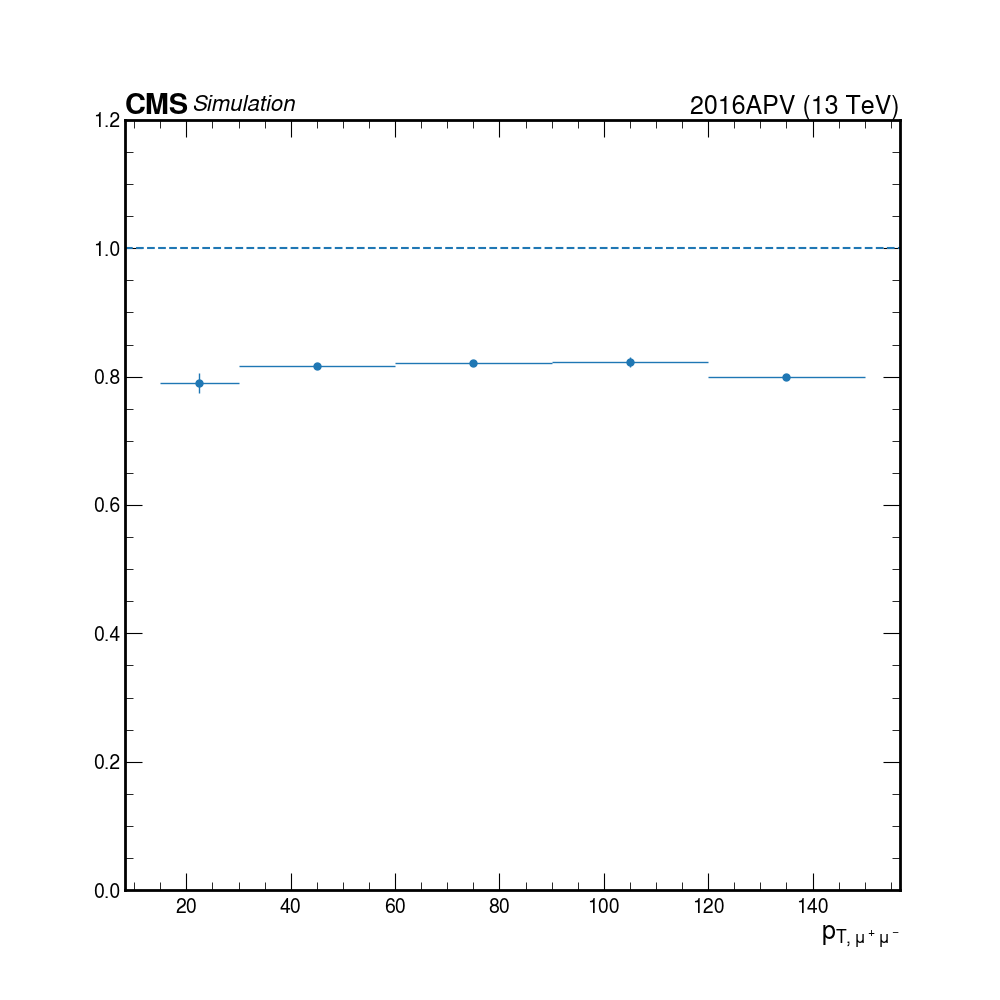
\includegraphics[width=0.44\textwidth]{figures/efficiency/acc_dimu_pt_2016APV.png}}}\hfill
  \subfloat[][]{\label{subfig:acc_dimu_rap_2016APV}%
    \fbox{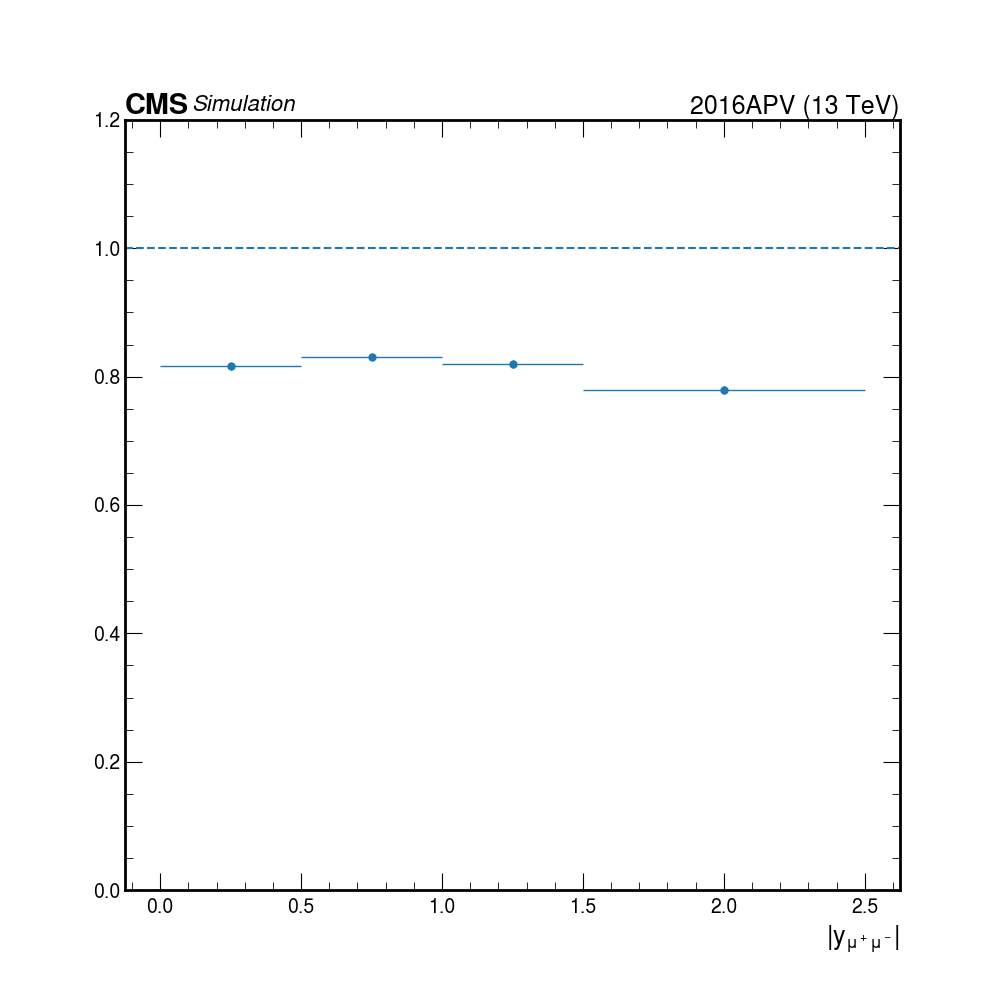
\includegraphics[width=0.44\textwidth]{figures/efficiency/acc_dimu_rap_2016APV.png}}}\hfill\\
  \subfloat[][]{\label{subfig:acc_dimu_2D_2016APV}%
    \fbox{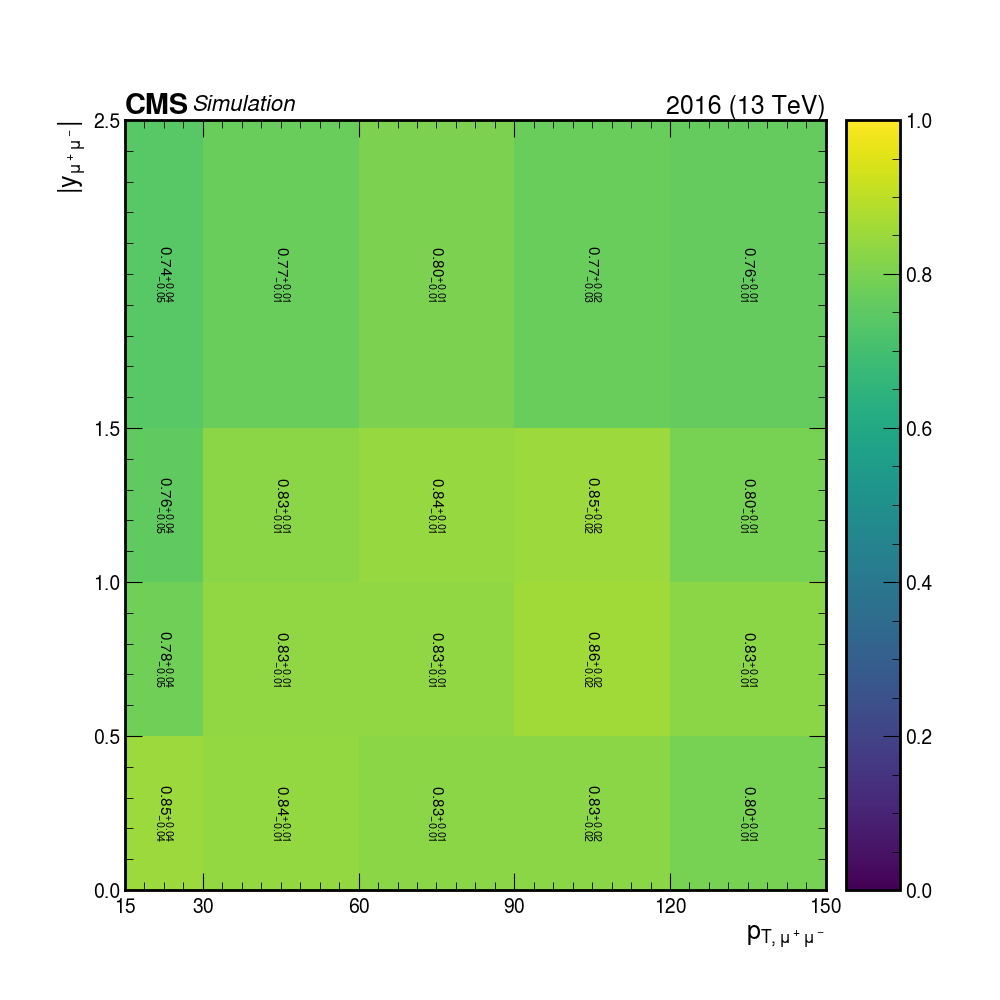
\includegraphics[width=0.44\textwidth]{figures/efficiency/acc_dimu_2016APV.png}}}\\
  \legend{$\Upsilon$ acceptance extracted from the 2016APV MC data sample. The acceptance is given with respect to the dimuon $p_T$ in (a), $y$ in (b), and in both $p_T$ and $y$ in (c). In (a) and (b). The horizontal dashed line is set to the upper limit of the acceptance, one.}
\end{figure}

\begin{figure}[H]{15cm}
  \caption{D$^*$ acceptance of the selected associated $\Upsilon +$ D$^*$ extracted from 2016APV MC sample.}
  \label{fig:acc_dstar_2016APV}
  \subfloat[][]{\label{subfig:acc_dstar_pt_2016APV}%
    \fbox{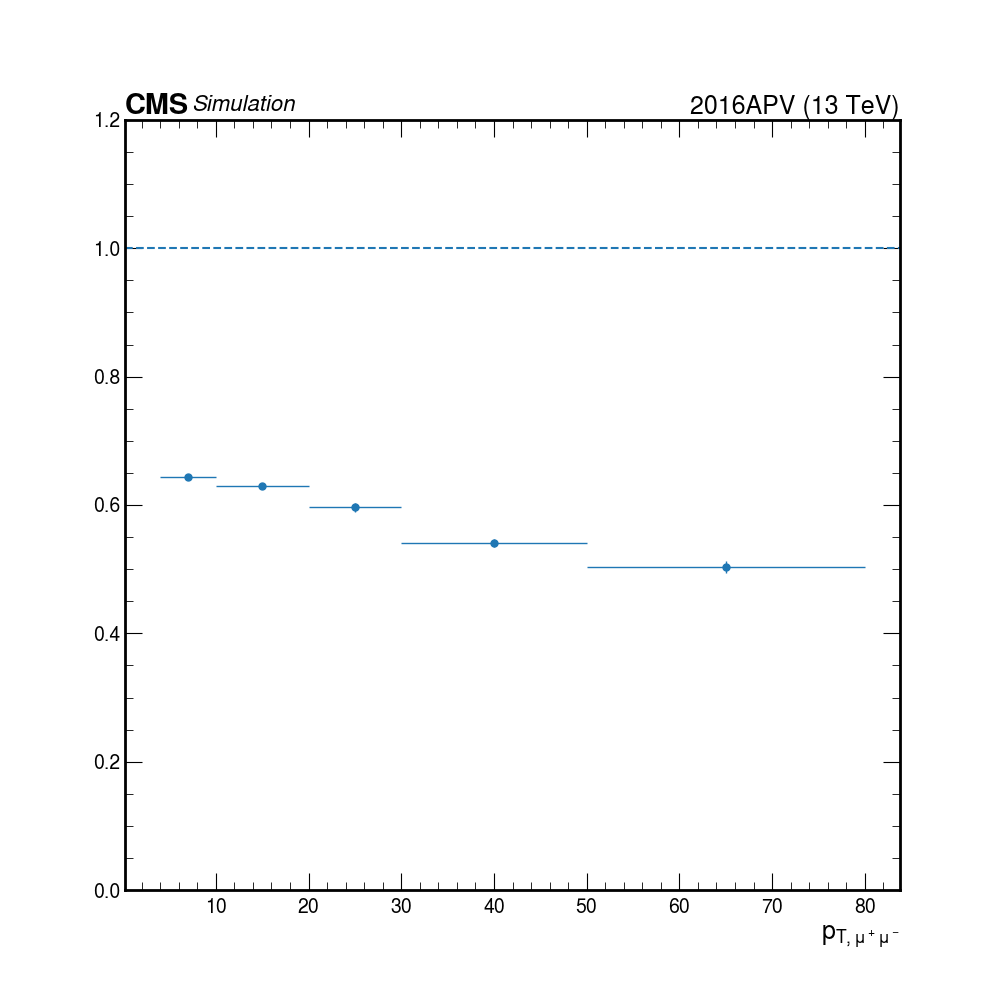
\includegraphics[width=0.44\textwidth]{figures/efficiency/acc_dstar_pt_2016APV.png}}}\hfill
  \subfloat[][]{\label{subfig:acc_dstar_rap_2016APV}%
    \fbox{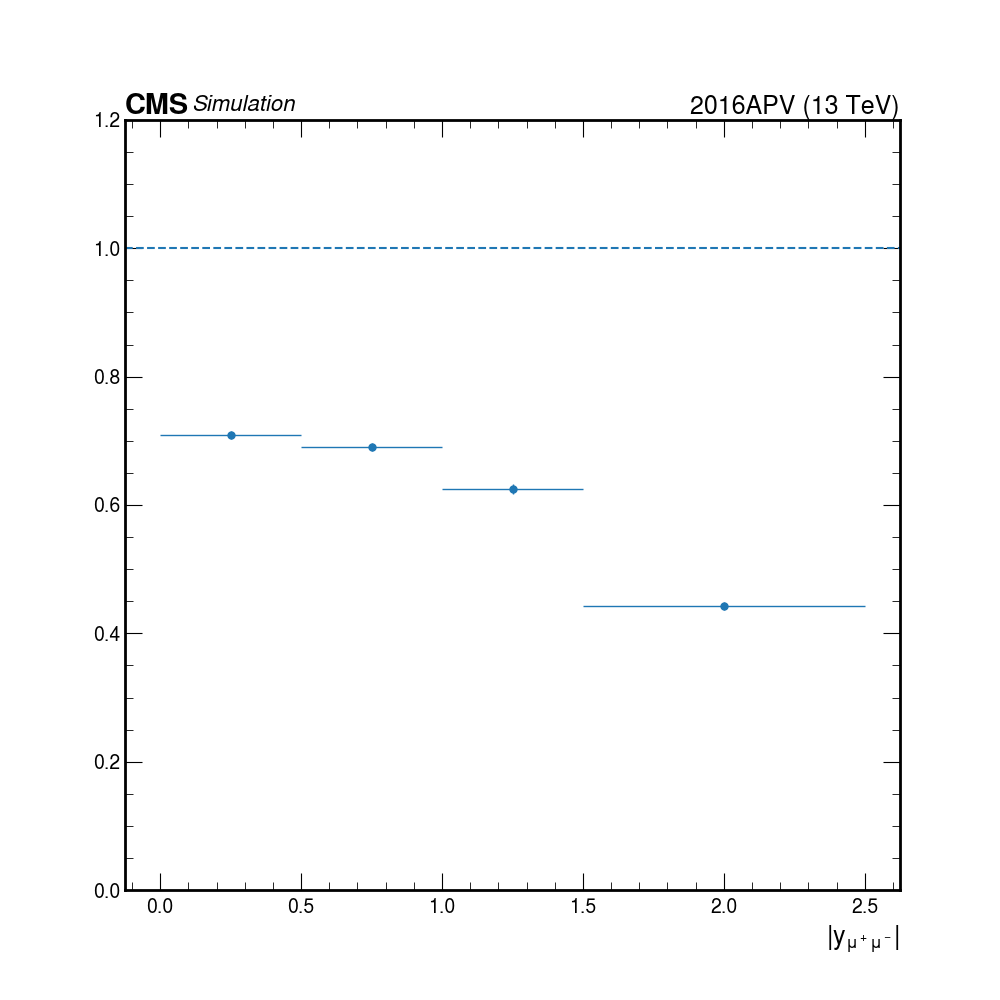
\includegraphics[width=0.44\textwidth]{figures/efficiency/acc_dstar_rap_2016APV.png}}}\hfill\\
  \subfloat[][]{\label{subfig:acc_dstar_2D_2016APV}%
    \fbox{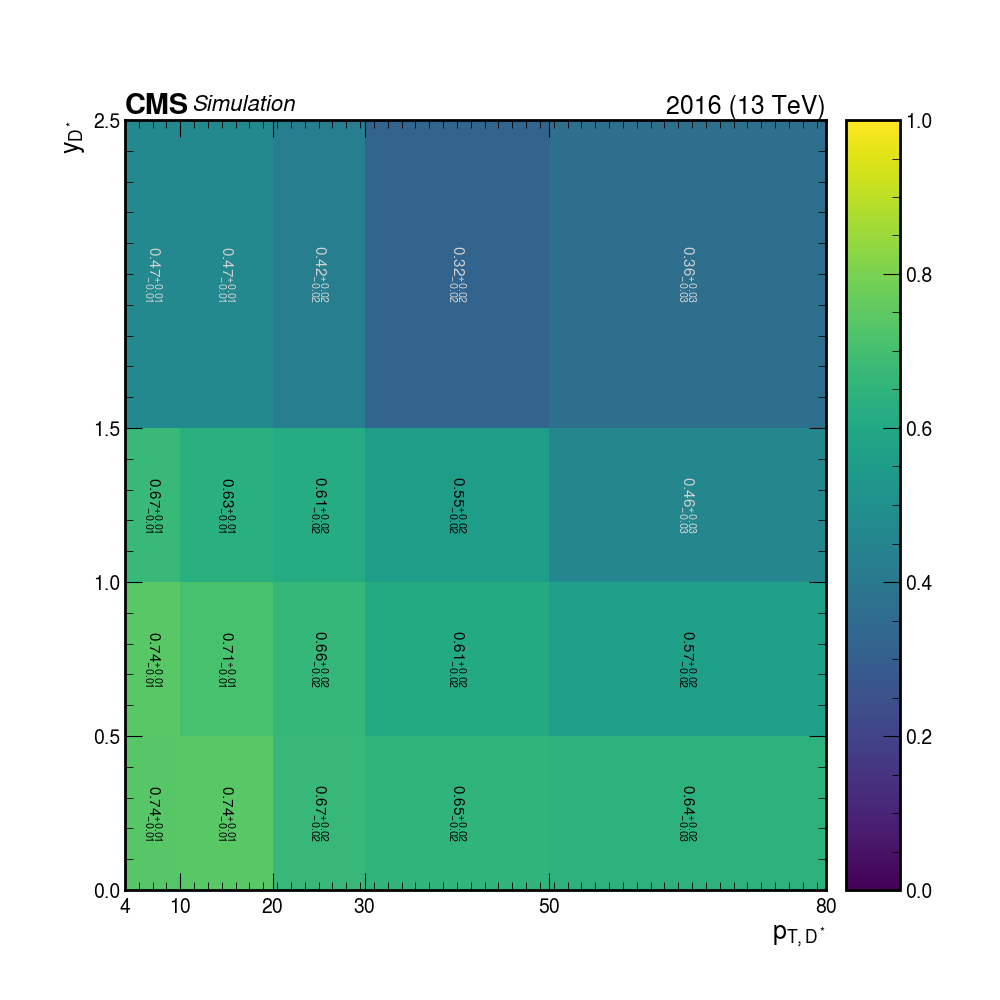
\includegraphics[width=0.44\textwidth]{figures/efficiency/acc_dstar_2016APV.png}}}\\
  \legend{D$^*$ acceptance extracted from the 2016APV MC data sample. The acceptance is given with respect to the reconstructed D$^*$ $p_T$ in (a), $y$ in (b), and in both $p_T$ and $y$ in (c). In (a) and (b). The horizontal dashed line is set to the upper limit of the acceptance, one.}
\end{figure}

\begin{figure}[H]{15cm}
  \caption{$\Upsilon$ selection cuts efficiency of the selected associated $\Upsilon +$ D$^*$ extracted from 2016APV MC sample.}
  \label{fig:eff_cuts_dimu_2016APV}
  \subfloat[][]{\label{subfig:eff_cuts_dimu_pt_2016APV}%
  \fbox{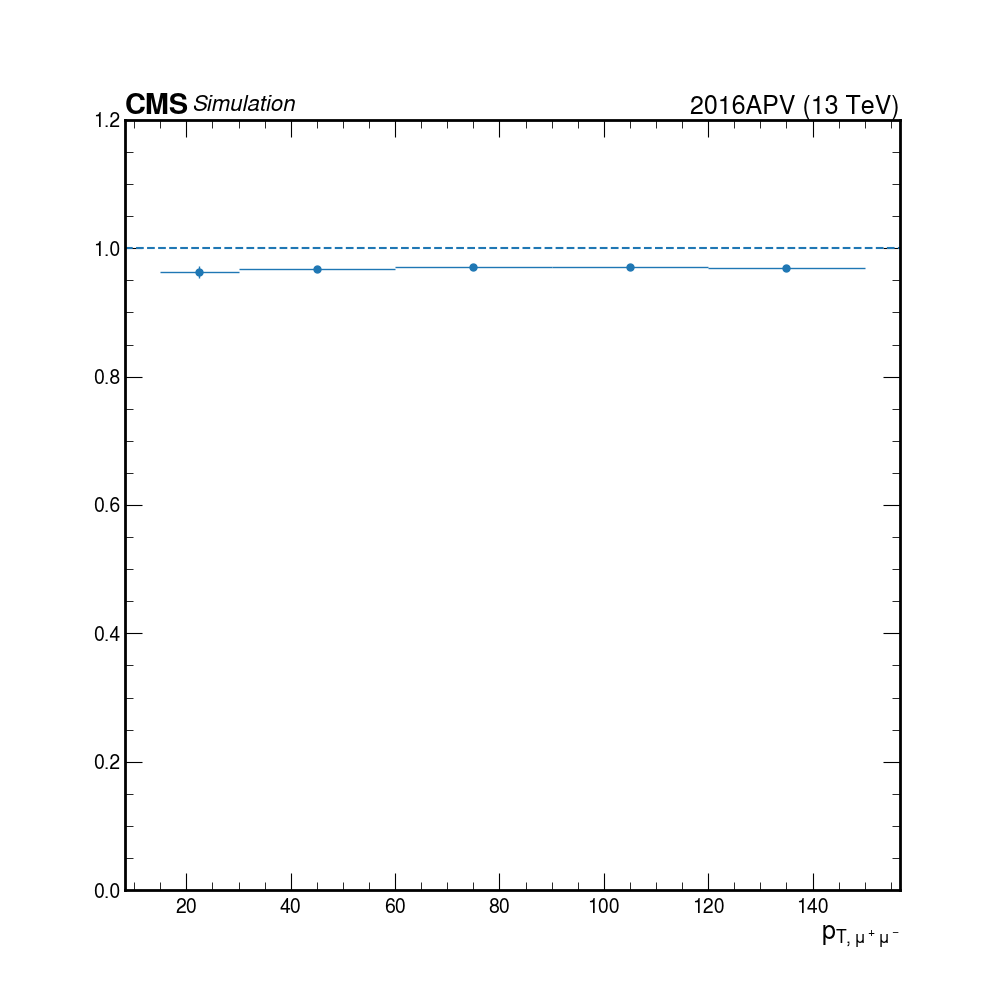
\includegraphics[width=0.44\textwidth]{figures/efficiency/eff_cuts_dimu_pt_2016APV.png}}}\hfill
  \subfloat[][]{\label{subfig:eff_cuts_dimu_rap_2016APV}%
  \fbox{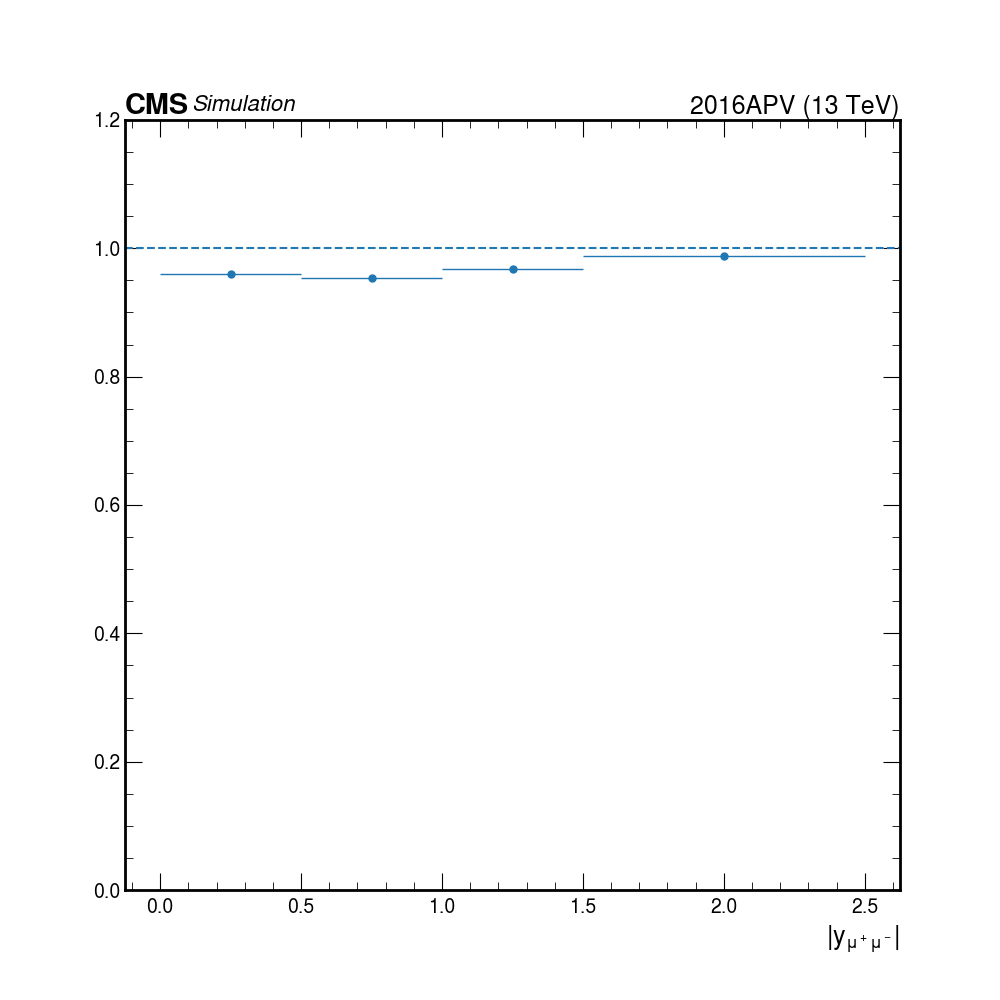
\includegraphics[width=0.44\textwidth]{figures/efficiency/eff_cuts_dimu_rap_2016APV.png}}}\hfill\\
  \subfloat[][]{\label{subfig:eff_cuts_dimu_2D_2016APV}%
  \fbox{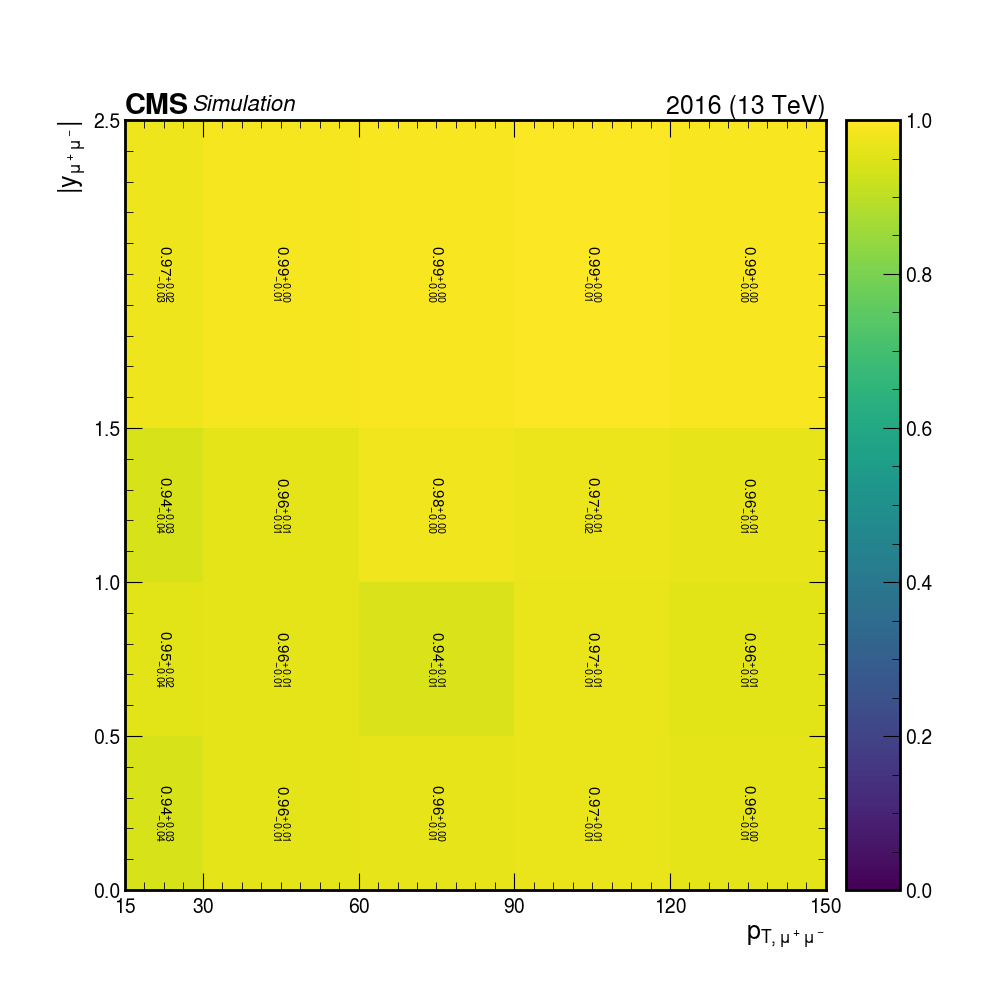
\includegraphics[width=0.44\textwidth]{figures/efficiency/eff_cuts_dimu_2016APV.png}}}\\
  \legend{$\Upsilon$ selection cuts efficiency extracted from the 2016APV MC data sample. This efficiency is given with respect to the dimuon $p_T$ in (a), $y$ in (b), and in both $p_T$ and $y$ in (c). In (a) and (b). The horizontal dashed line is set to the upper limit of the efficiency.}
\end{figure}

\begin{figure}[H]{15cm}
  \caption{D$^*$ selection cuts efficiency of the selected associated $\Upsilon +$ D$^*$ extracted from 2016APV MC sample.}
  \label{fig:eff_cuts_dstar_2016APV}
  \subfloat[][]{\label{subfig:eff_cuts_dstar_pt_2016APV}%
    \fbox{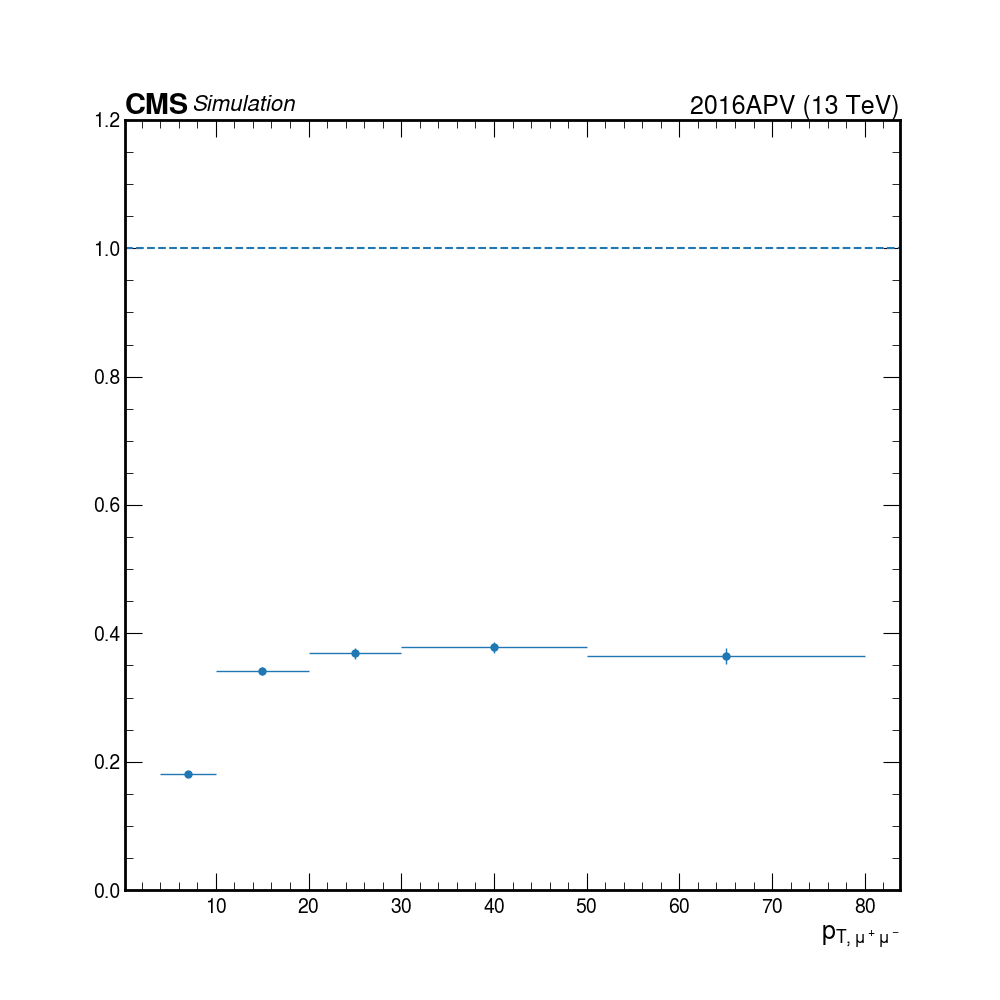
\includegraphics[width=0.44\textwidth]{figures/efficiency/eff_cuts_dstar_pt_2016APV.png}}}\hfill
  \subfloat[][]{\label{subfig:eff_cuts_dstar_rap_2016APV}%
    \fbox{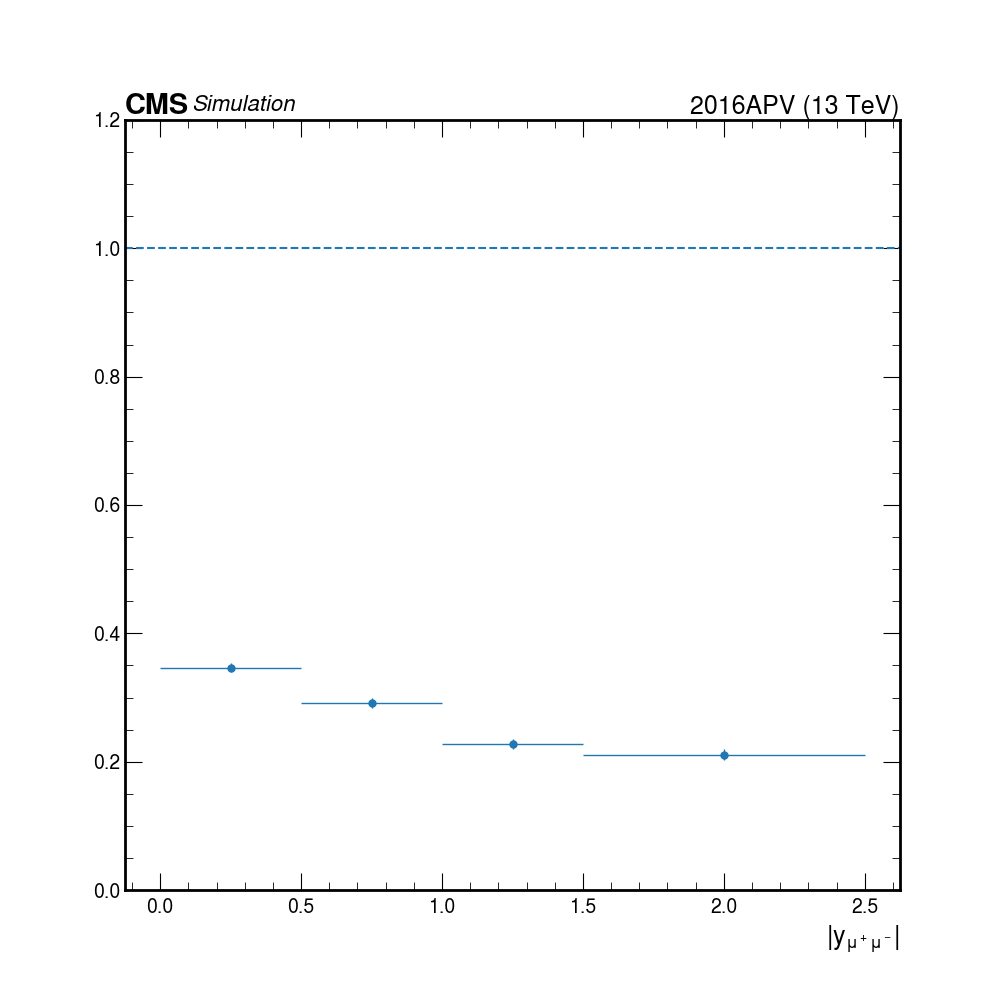
\includegraphics[width=0.44\textwidth]{figures/efficiency/eff_cuts_dstar_rap_2016APV.png}}}\hfill\\
  \subfloat[][]{\label{subfig:eff_cuts_dstar_2D_2016APV}%
    \fbox{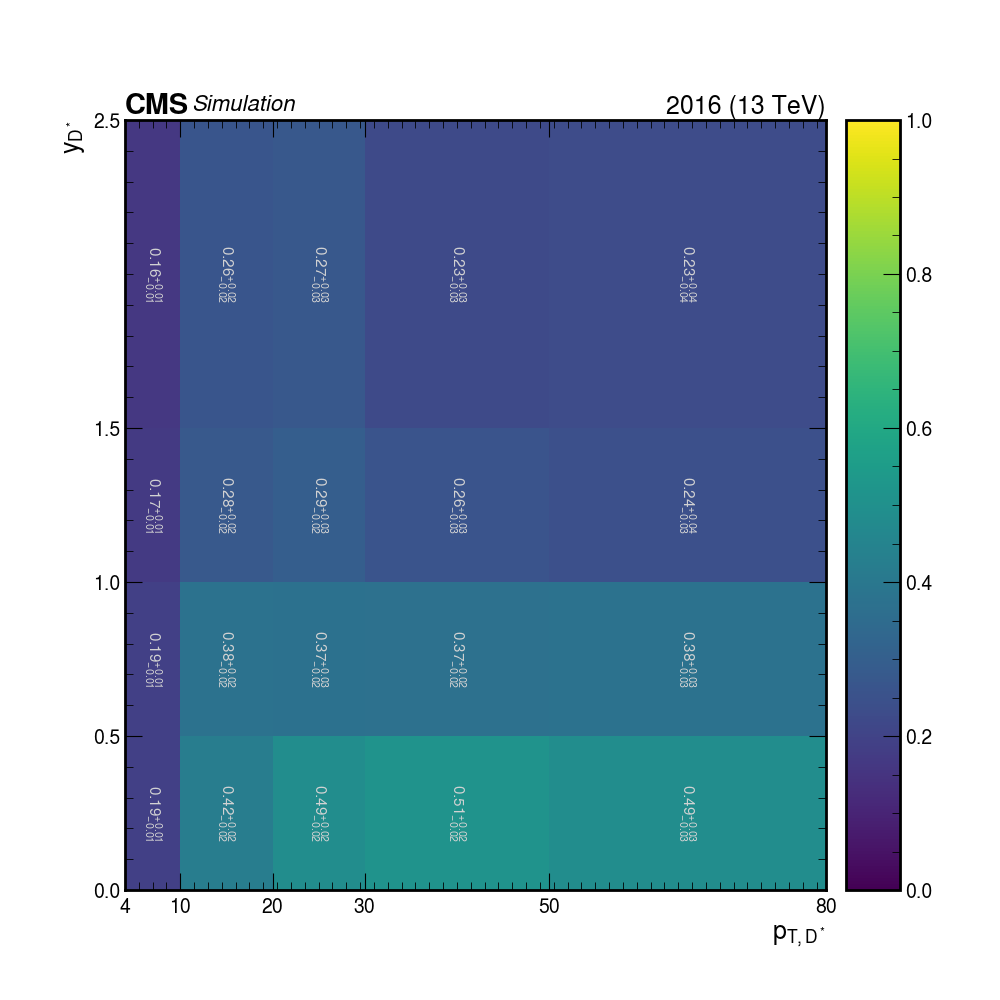
\includegraphics[width=0.44\textwidth]{figures/efficiency/eff_cuts_dstar_2016APV.png}}}\\
  \legend{D$^*$ selection cuts efficiency extracted from the 2016APV MC data sample. This efficiency is given with respect to the D$^*$ $p_T$ in (a), $y$ in (b), and in both $p_T$ and $y$ in (c). In (a) and (b). The horizontal dashed line is set to the upper limit of the efficiency.}
\end{figure}

\begin{figure}[H]{15cm}
  \caption{Trigger efficiency of the selected associated $\Upsilon +$ D$^*$ extracted from 2016APV MC sample.}
  \label{fig:eff_trigger_2016APV}
  \subfloat[][]{\label{subfig:eff_trigger_pt_2016APV}%
    \fbox{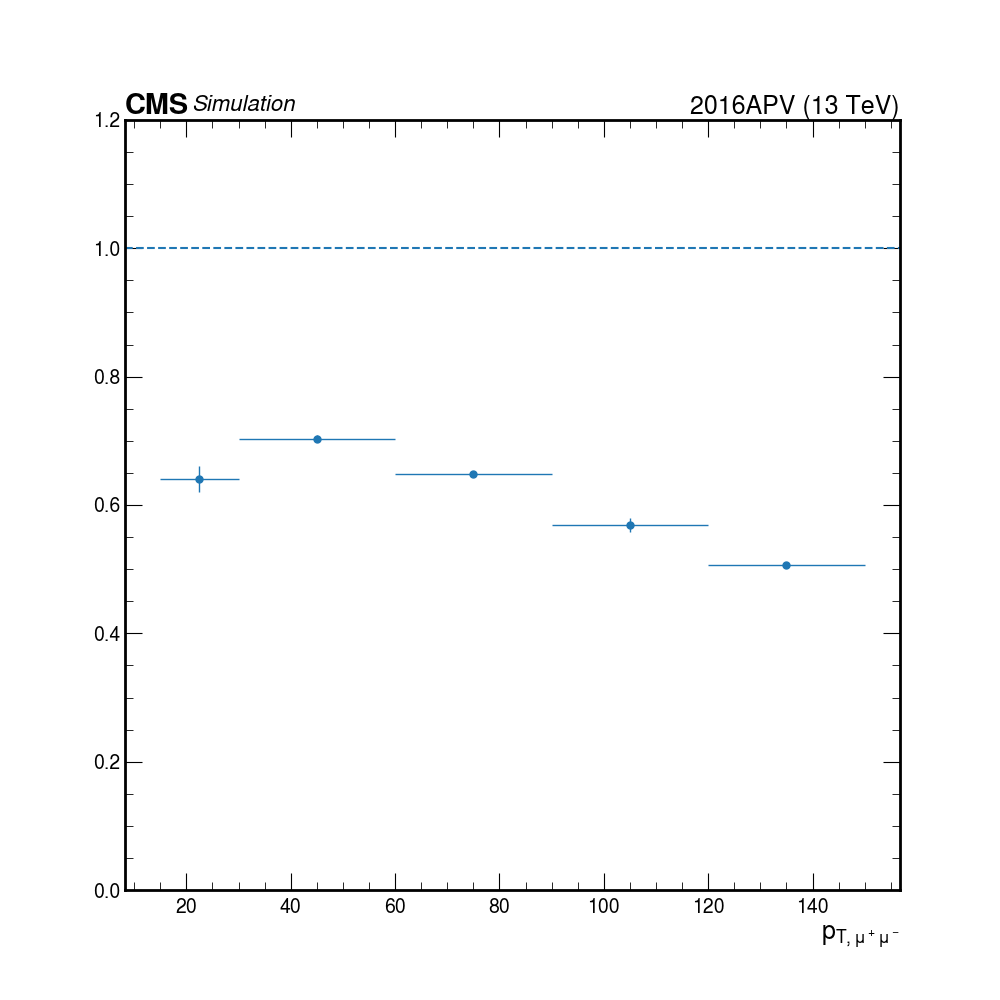
\includegraphics[width=0.44\textwidth]{figures/efficiency/eff_trigger_pt_2016APV.png}}}\hfill
  \subfloat[][]{\label{subfig:eff_trigger_rap_2016APV}%
    \fbox{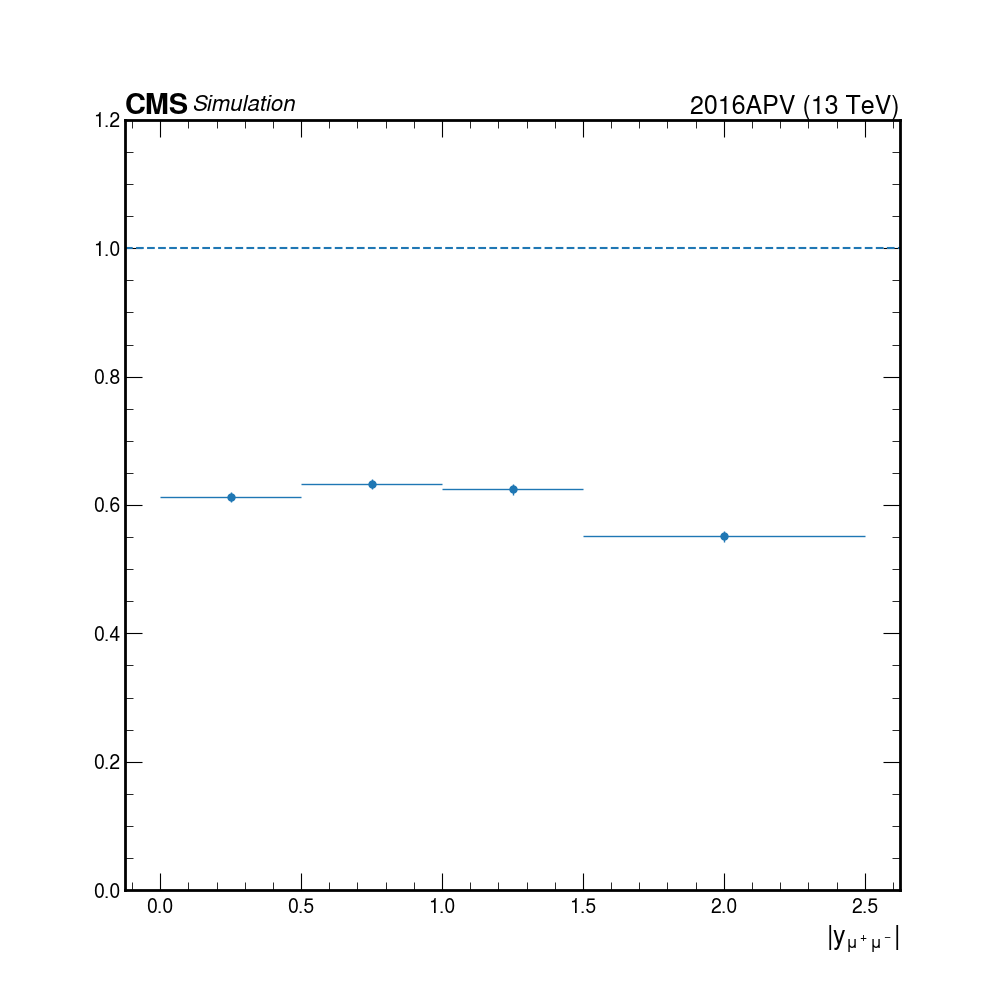
\includegraphics[width=0.44\textwidth]{figures/efficiency/eff_trigger_rap_2016APV.png}}}\hfill\\
  \subfloat[][]{\label{subfig:eff_trigger_2D_2016APV}%
    \fbox{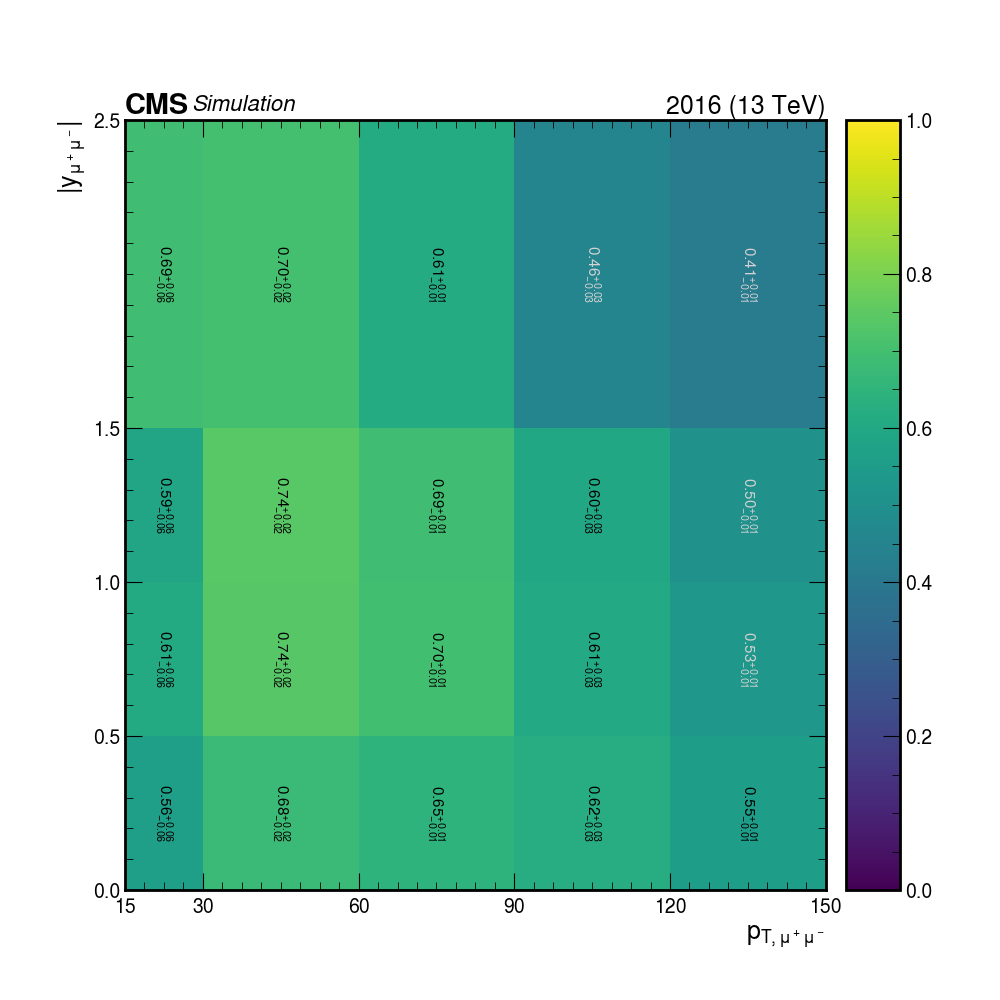
\includegraphics[width=0.44\textwidth]{figures/efficiency/eff_trigger_2016APV.png}}}\\
  \legend{Trigger efficiency extracted from the 2016APV MC data sample. This efficiency is given with respect to the dimuon $p_T$ in (a), $y$ in (b), and in both $p_T$ and $y$ in (c). In (a) and (b). The horizontal dashed line is set to the upper limit of the efficiency.}
\end{figure}

\begin{figure}[H]{15cm}
  \caption{Trigger efficiency of the selected associated $\Upsilon +$ D$^*$ extracted from 2016APV MC sample.}
  \label{fig:eff_asso_2016APV}
  \subfloat[][]{\label{subfig:eff_asso_pt_2016APV}%
    \fbox{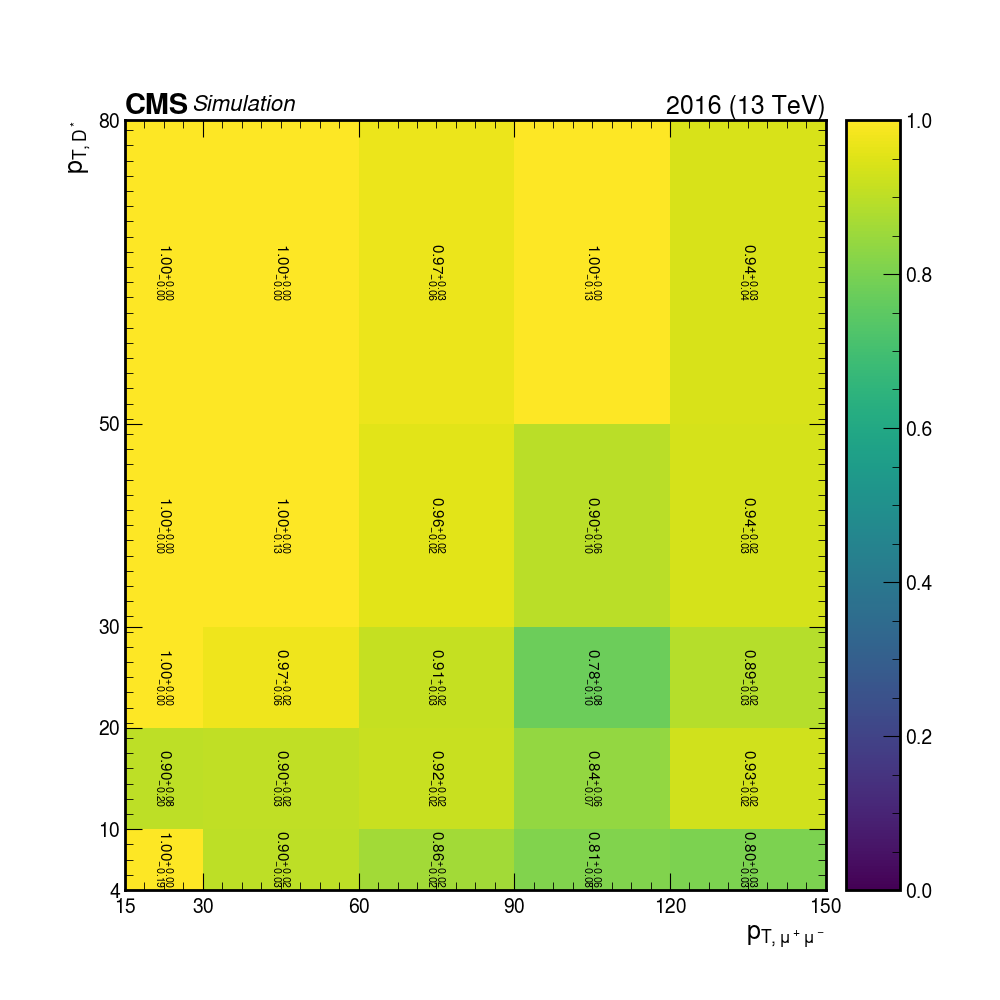
\includegraphics[width=0.44\textwidth]{figures/efficiency/eff_asso_pt_2016APV.png}}}\hfill
  \subfloat[][]{\label{subfig:eff_asso_rap_2016APV}%
    \fbox{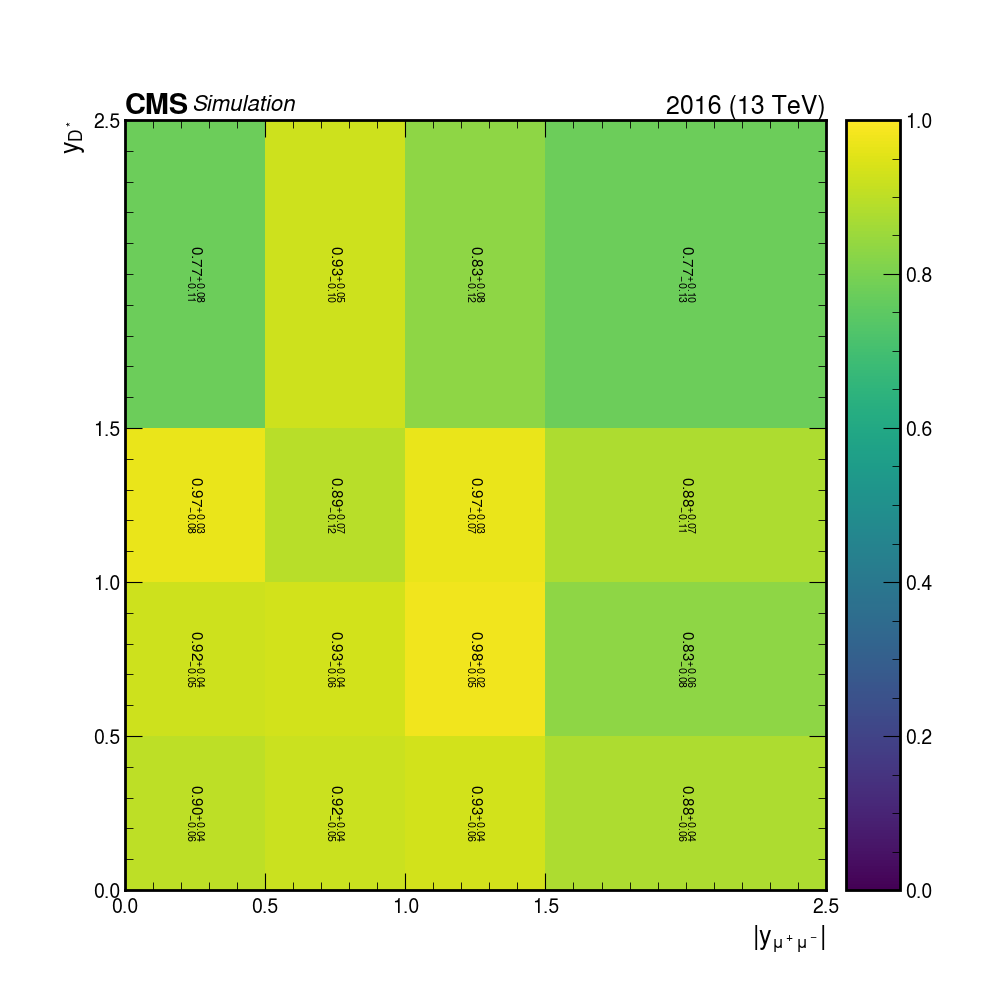
\includegraphics[width=0.44\textwidth]{figures/efficiency/eff_asso_rap_2016APV.png}}}\hfill\\
  \legend{Association efficiency extracted from the 2016APV MC data sample. The efficiency maps are given with respect to the dimuon and D$^*$ $p_T$ in (a) and $y$ in (b).}
\end{figure}

\clearpage

\section{Efficiencies for sample 2016}

\begin{figure}[H]{15cm}
  \caption{$\Upsilon$ acceptance of the selected associated $\Upsilon +$ D$^*$ extracted from 2016 MC sample.}
  \label{fig:acc_dimu_2016}
  \subfloat[][]{\label{subfig:acc_dimu_pt_2016}%
    \fbox{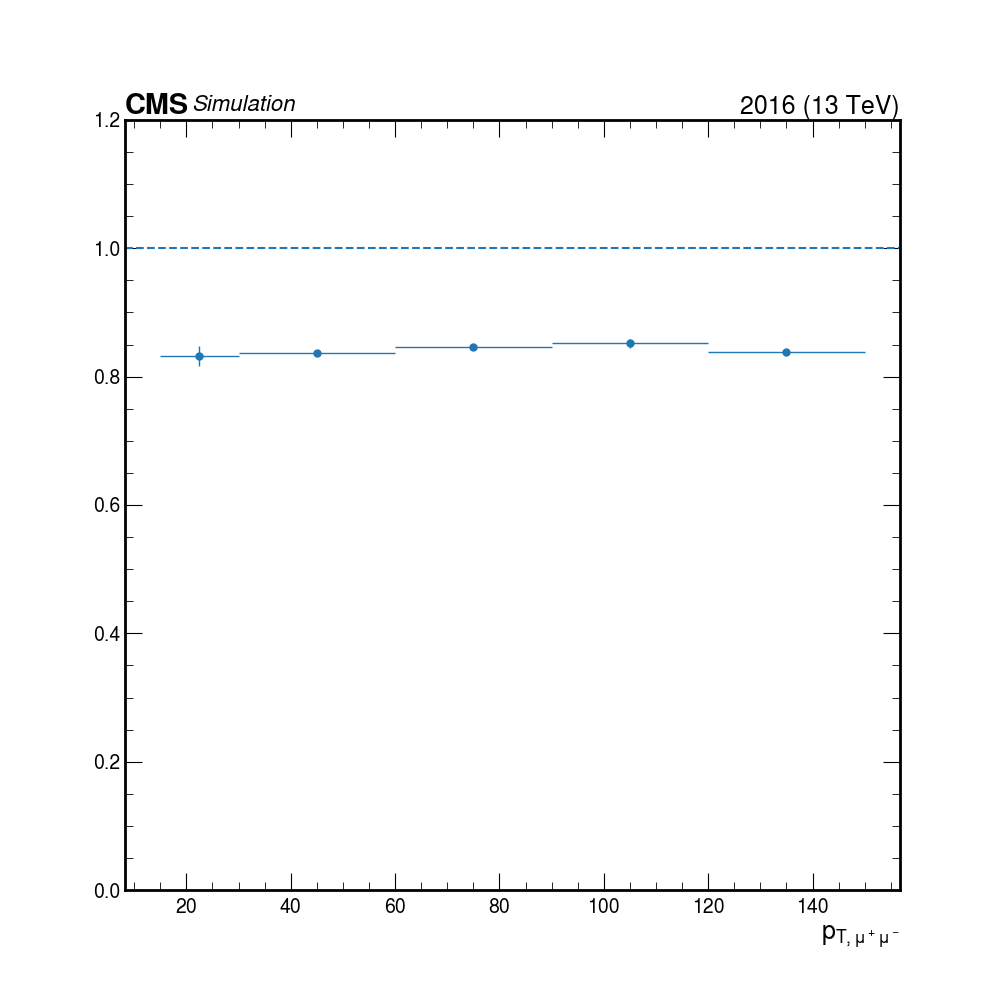
\includegraphics[width=0.44\textwidth]{figures/efficiency/acc_dimu_pt_2016.png}}}\hfill
  \subfloat[][]{\label{subfig:acc_dimu_rap_2016}%
    \fbox{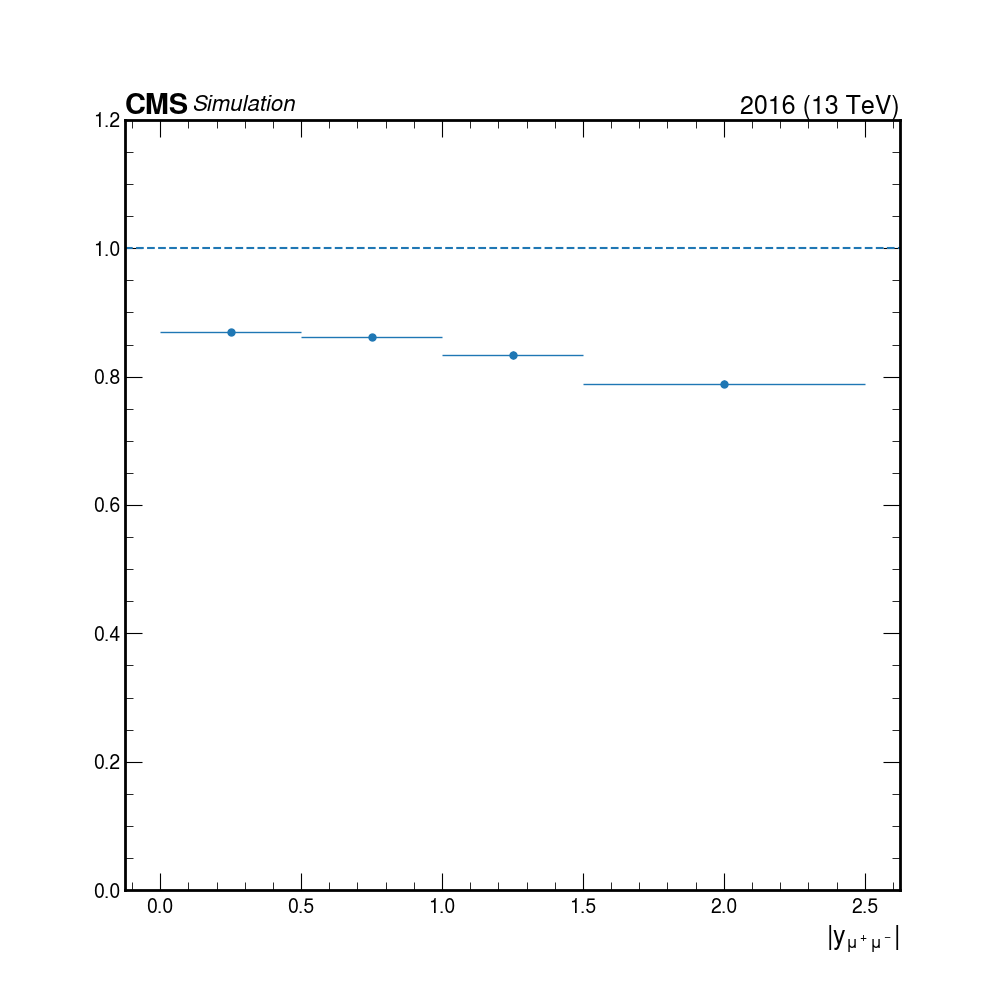
\includegraphics[width=0.44\textwidth]{figures/efficiency/acc_dimu_rap_2016.png}}}\hfill\\
  \subfloat[][]{\label{subfig:acc_dimu_2D_2016}%
    \fbox{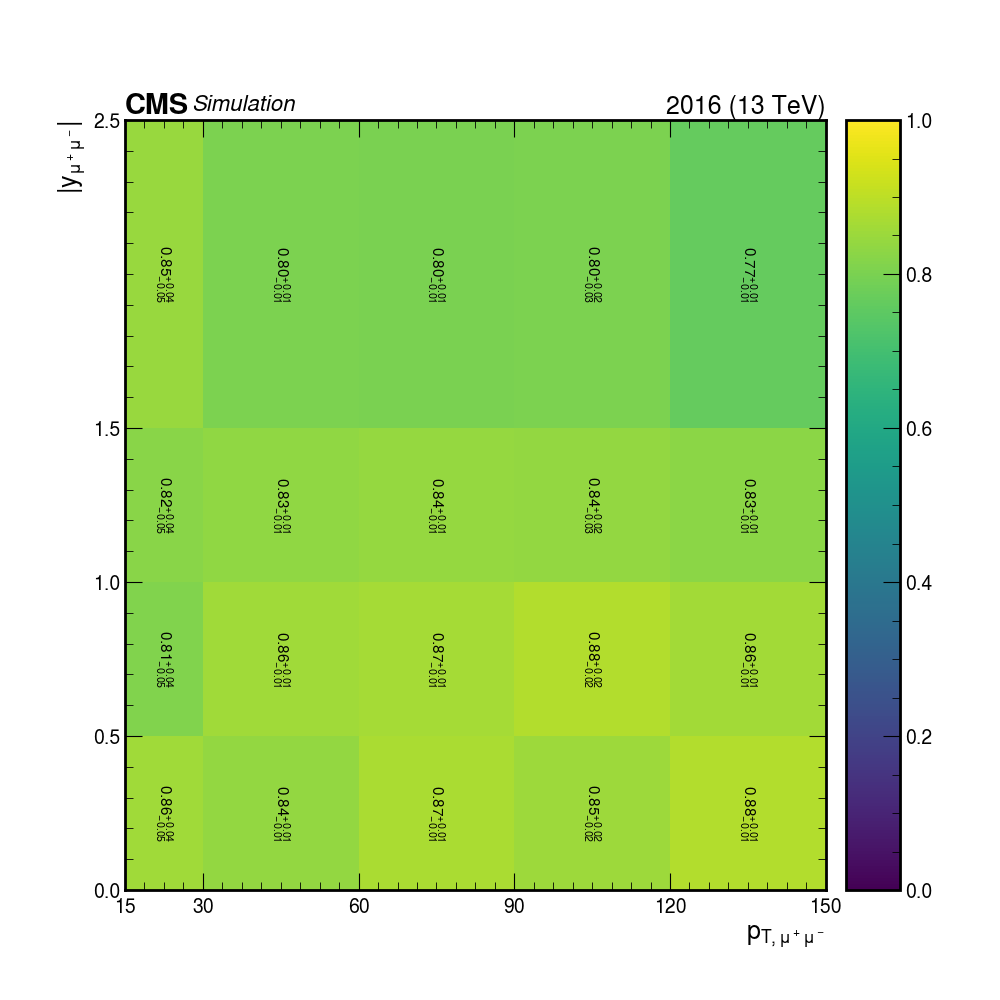
\includegraphics[width=0.44\textwidth]{figures/efficiency/acc_dimu_2016.png}}}\\
  \legend{$\Upsilon$ acceptance extracted from the 2016 MC data sample. The acceptance is given with respect to the dimuon $p_T$ in (a), $y$ in (b), and in both $p_T$ and $y$ in (c). In (a) and (b). The horizontal dashed line is set to the upper limit of the acceptance, one.}
\end{figure}

\begin{figure}[H]{15cm}
  \caption{D$^*$ acceptance of the selected associated $\Upsilon +$ D$^*$ extracted from 2016 MC sample.}
  \label{fig:acc_dstar_2016}
  \subfloat[][]{\label{subfig:acc_dstar_pt_2016}%
    \fbox{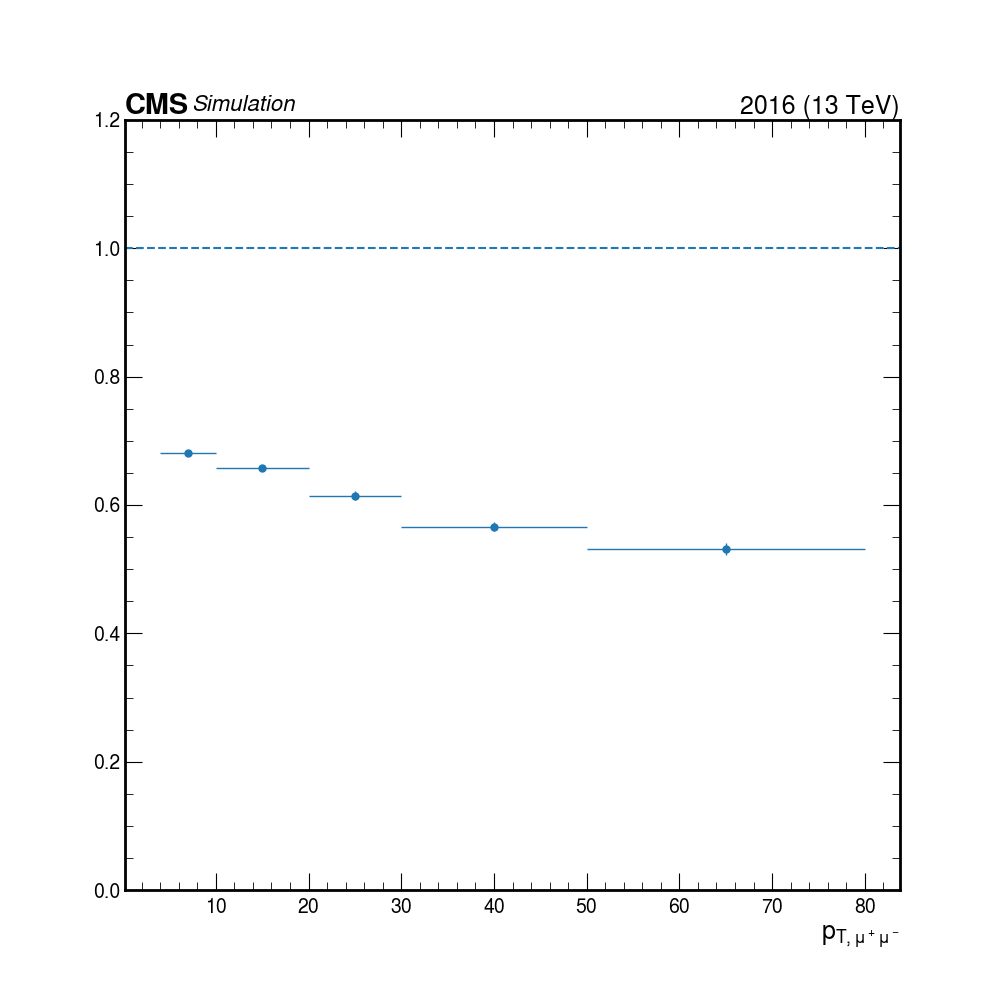
\includegraphics[width=0.44\textwidth]{figures/efficiency/acc_dstar_pt_2016.png}}}\hfill
  \subfloat[][]{\label{subfig:acc_dstar_rap_2016}%
    \fbox{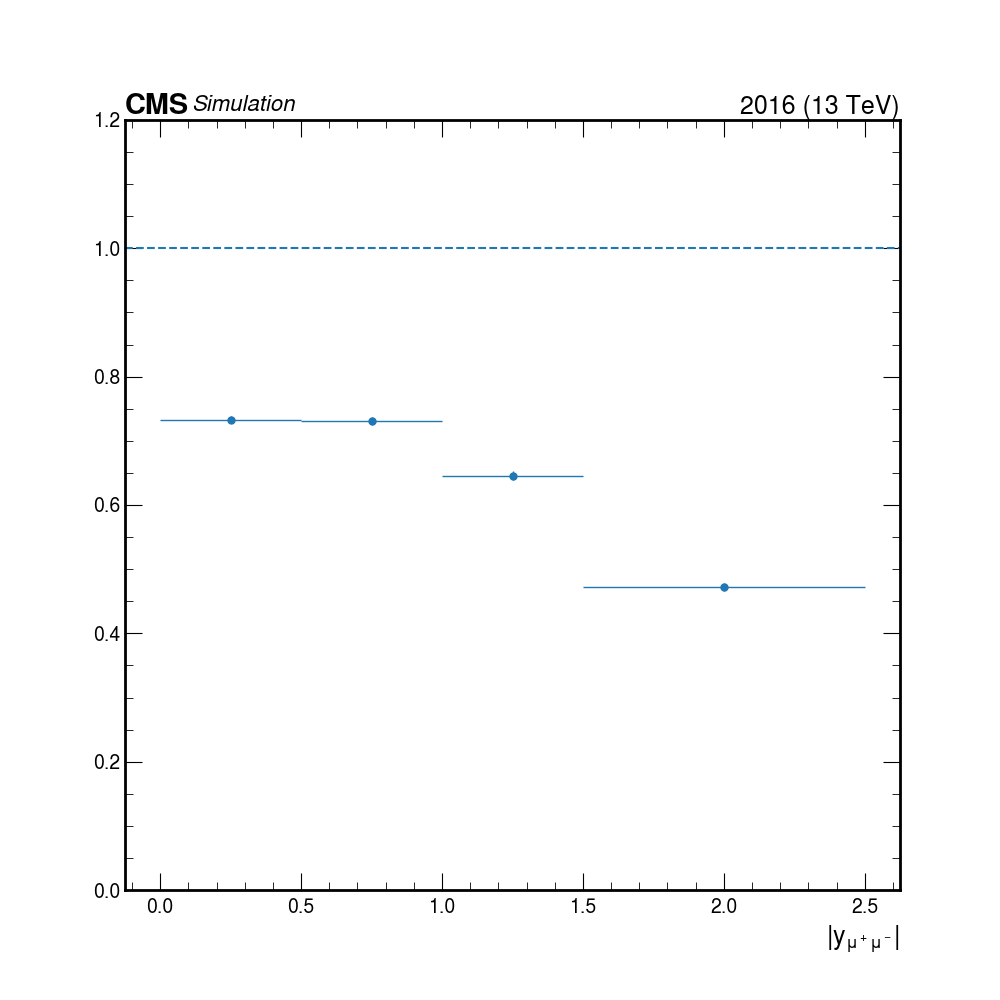
\includegraphics[width=0.44\textwidth]{figures/efficiency/acc_dstar_rap_2016.png}}}\hfill\\
  \subfloat[][]{\label{subfig:acc_dstar_2D_2016}%
    \fbox{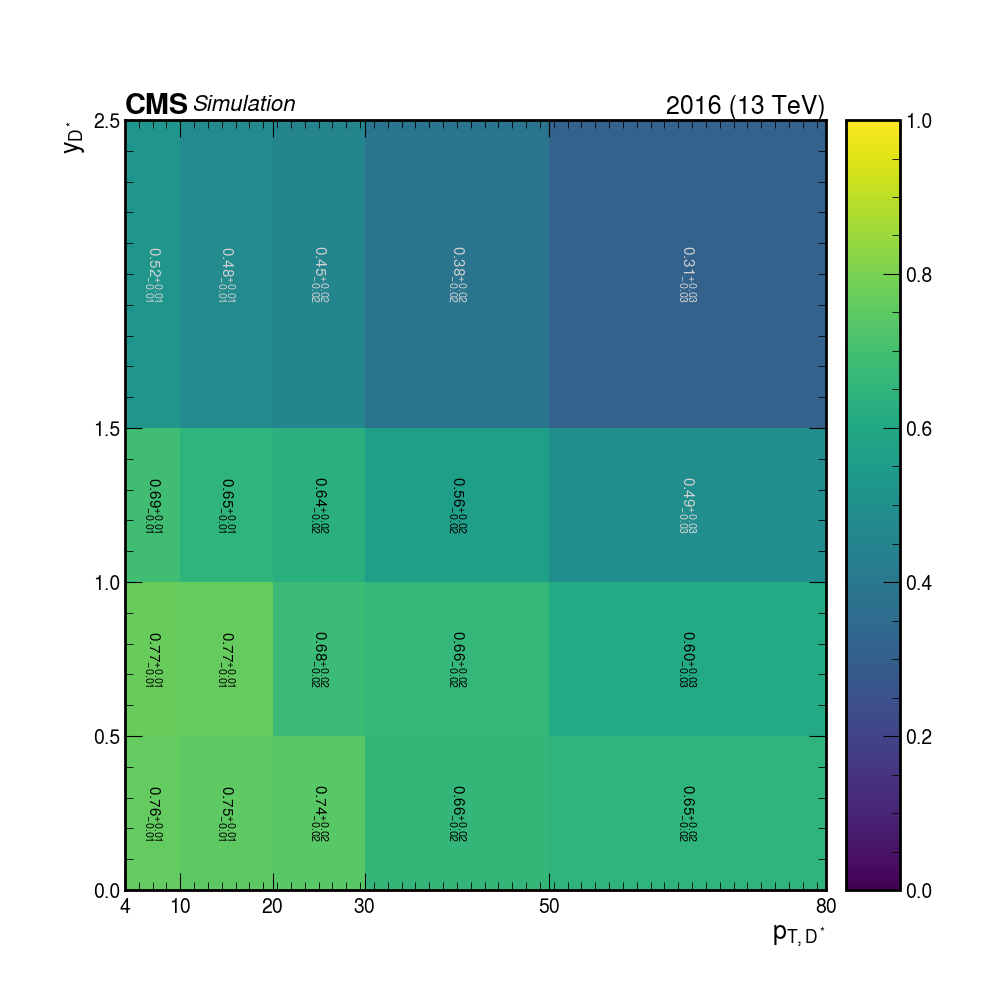
\includegraphics[width=0.44\textwidth]{figures/efficiency/acc_dstar_2016.png}}}\\
  \legend{D$^*$ acceptance extracted from the 2016 MC data sample. The acceptance is given with respect to the reconstructed D$^*$ $p_T$ in (a), $y$ in (b), and in both $p_T$ and $y$ in (c). In (a) and (b). The horizontal dashed line is set to the upper limit of the acceptance, one.}
\end{figure}

\begin{figure}[H]{15cm}
  \caption{$\Upsilon$ selection cuts efficiency of the selected associated $\Upsilon +$ D$^*$ extracted from 2016 MC sample.}
  \label{fig:eff_cuts_dimu_2016}
  \subfloat[][]{\label{subfig:eff_cuts_dimu_pt_2016}%
  \fbox{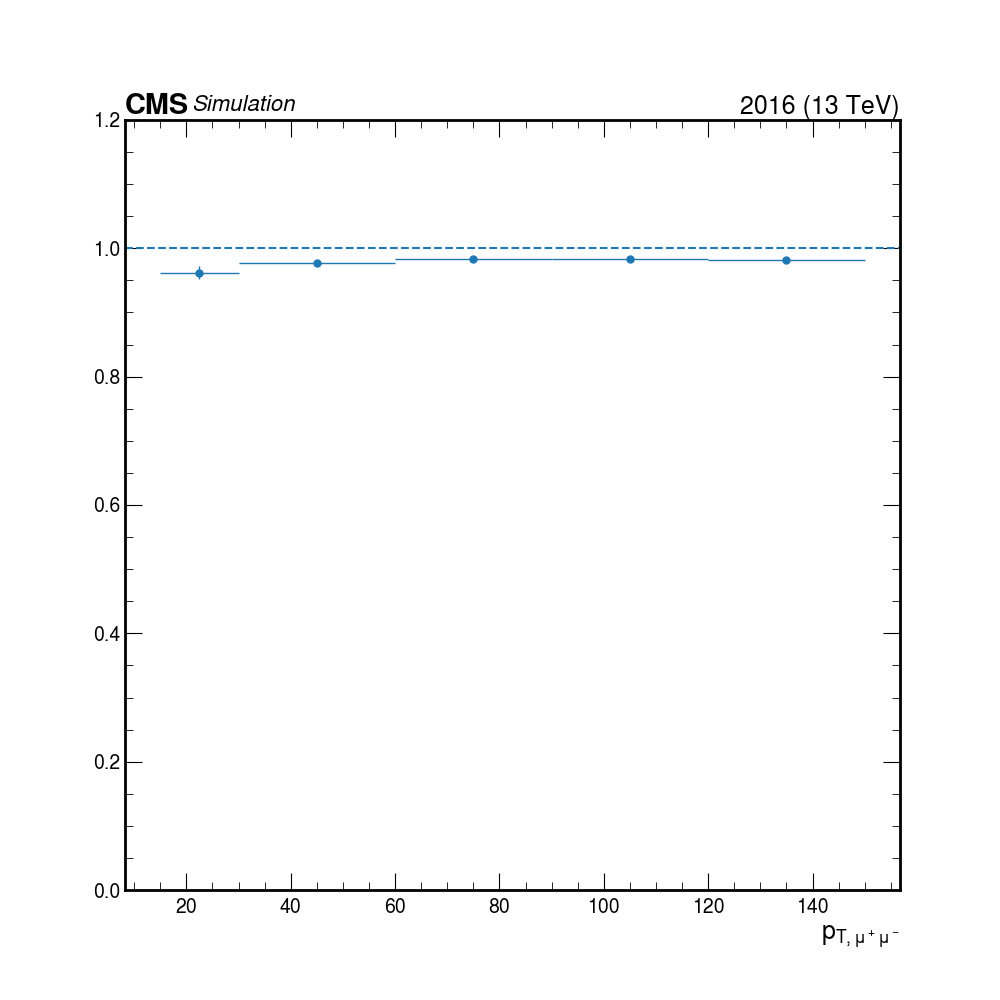
\includegraphics[width=0.44\textwidth]{figures/efficiency/eff_cuts_dimu_pt_2016.png}}}\hfill
  \subfloat[][]{\label{subfig:eff_cuts_dimu_rap_2016}%
  \fbox{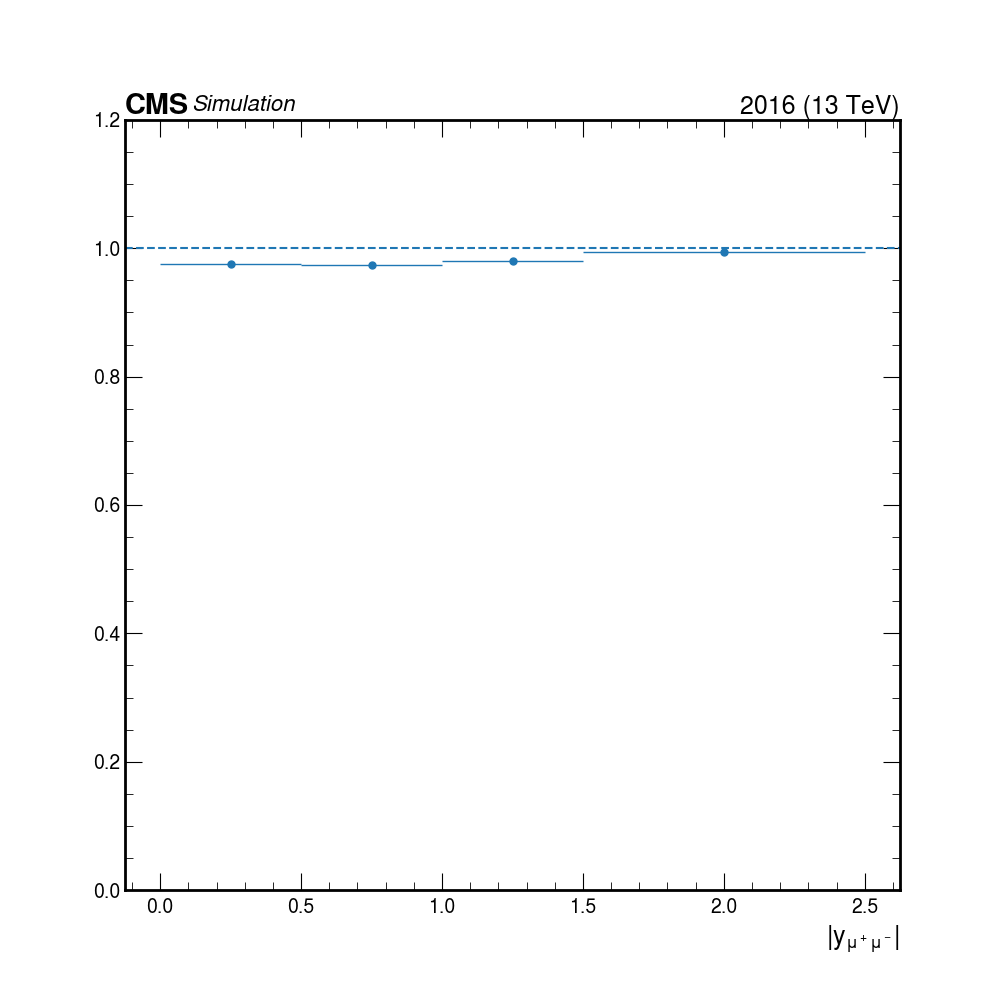
\includegraphics[width=0.44\textwidth]{figures/efficiency/eff_cuts_dimu_rap_2016.png}}}\hfill\\
  \subfloat[][]{\label{subfig:eff_cuts_dimu_2D_2016}%
  \fbox{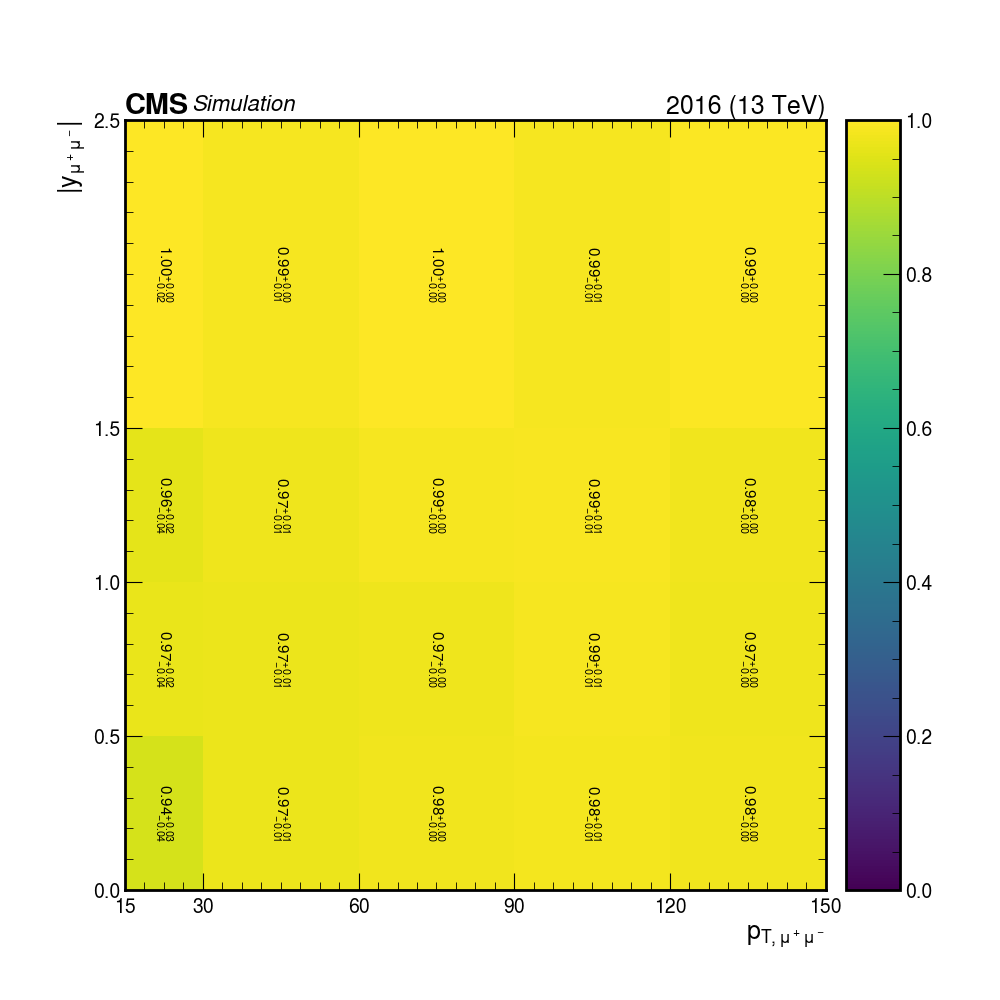
\includegraphics[width=0.44\textwidth]{figures/efficiency/eff_cuts_dimu_2016.png}}}\\
  \legend{$\Upsilon$ selection cuts efficiency extracted from the 2016 MC data sample. This efficiency is given with respect to the dimuon $p_T$ in (a), $y$ in (b), and in both $p_T$ and $y$ in (c). In (a) and (b). The horizontal dashed line is set to the upper limit of the efficiency.}
\end{figure}

\begin{figure}[H]{15cm}
  \caption{D$^*$ selection cuts efficiency of the selected associated $\Upsilon +$ D$^*$ extracted from 2016 MC sample.}
  \label{fig:eff_cuts_dstar_2016}
  \subfloat[][]{\label{subfig:eff_cuts_dstar_pt_2016}%
    \fbox{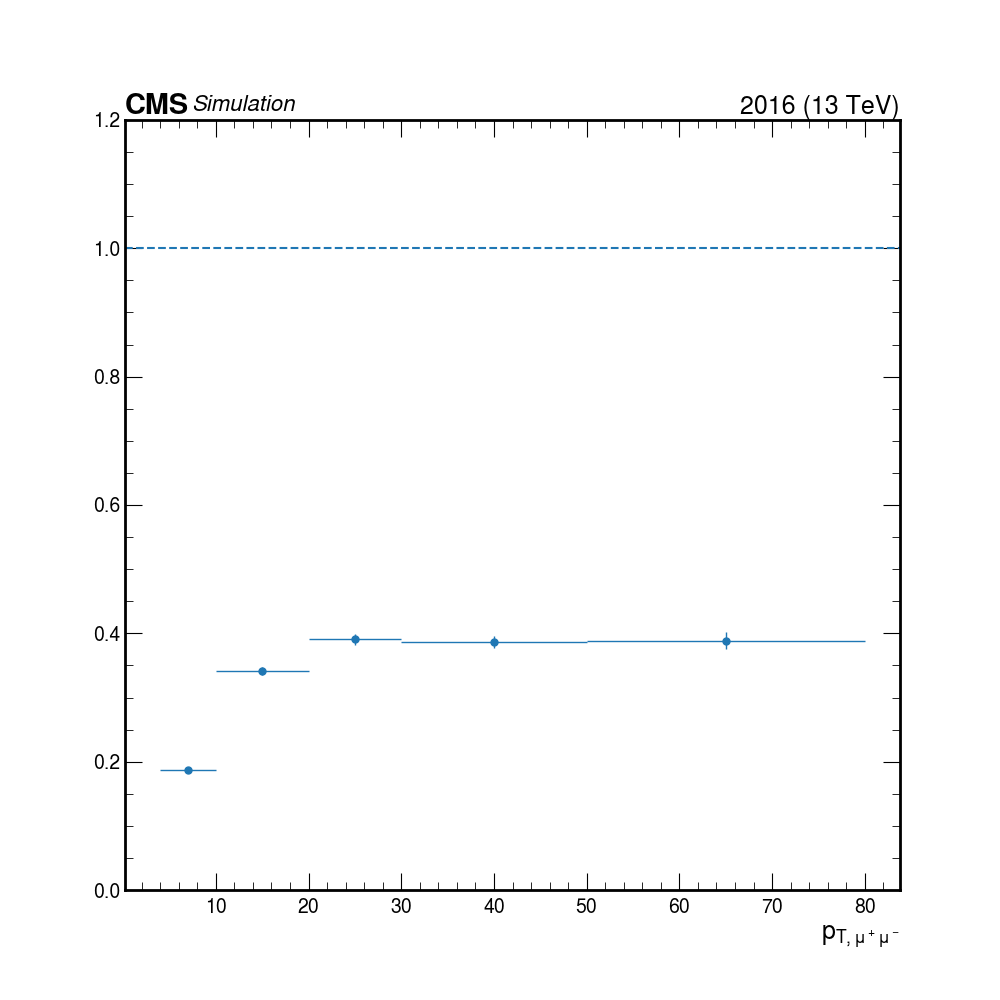
\includegraphics[width=0.44\textwidth]{figures/efficiency/eff_cuts_dstar_pt_2016.png}}}\hfill
  \subfloat[][]{\label{subfig:eff_cuts_dstar_rap_2016}%
    \fbox{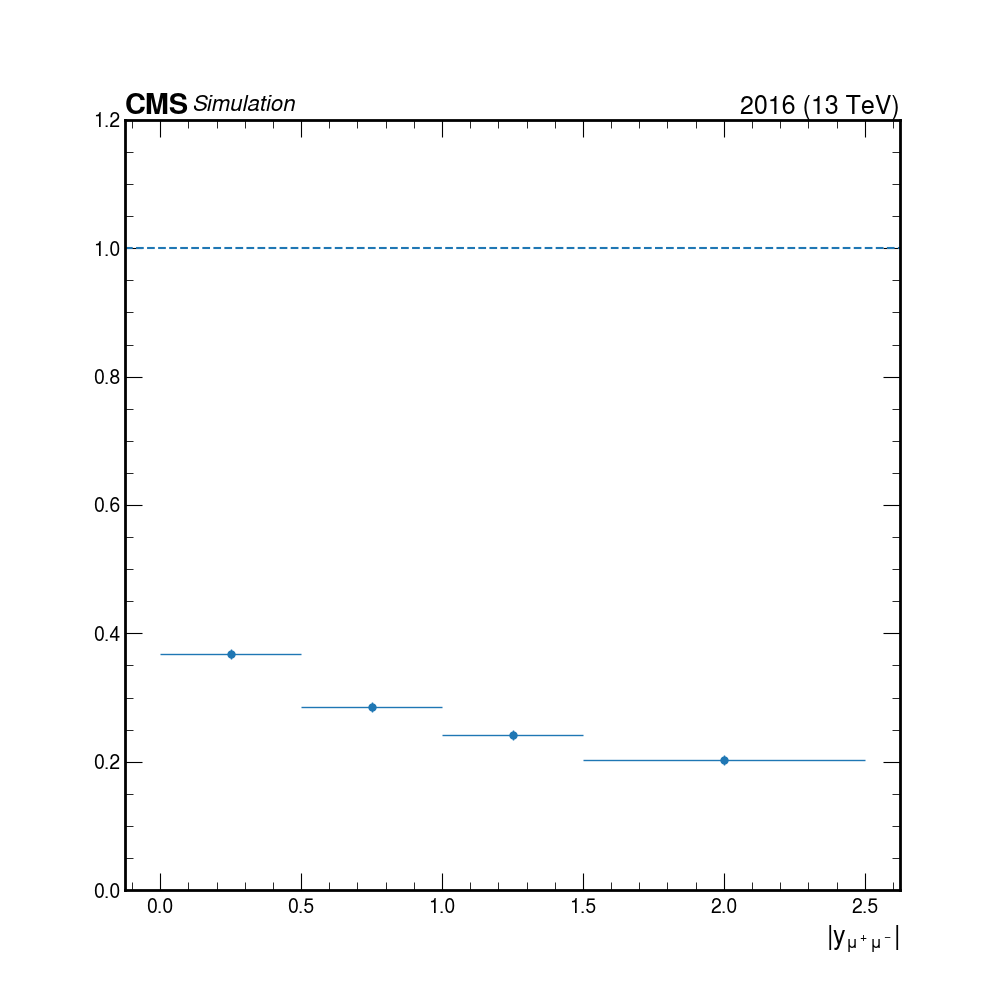
\includegraphics[width=0.44\textwidth]{figures/efficiency/eff_cuts_dstar_rap_2016.png}}}\hfill\\
  \subfloat[][]{\label{subfig:eff_cuts_dstar_2D_2016}%
    \fbox{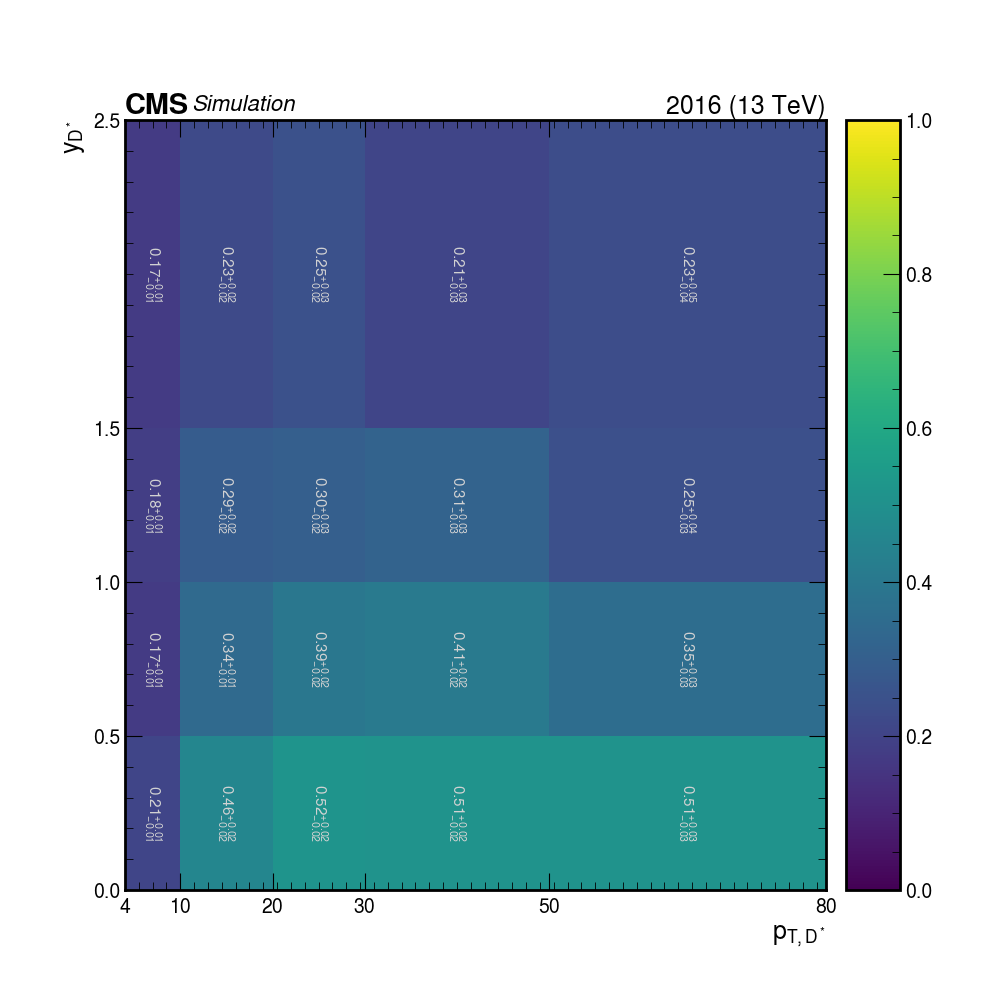
\includegraphics[width=0.44\textwidth]{figures/efficiency/eff_cuts_dstar_2016.png}}}\\
  \legend{D$^*$ selection cuts efficiency extracted from the 2016 MC data sample. This efficiency is given with respect to the D$^*$ $p_T$ in (a), $y$ in (b), and in both $p_T$ and $y$ in (c). In (a) and (b). The horizontal dashed line is set to the upper limit of the efficiency.}
\end{figure}

\begin{figure}[H]{15cm}
  \caption{Trigger efficiency of the selected associated $\Upsilon +$ D$^*$ extracted from 2016 MC sample.}
  \label{fig:eff_trigger_2016}
  \subfloat[][]{\label{subfig:eff_trigger_pt_2016}%
    \fbox{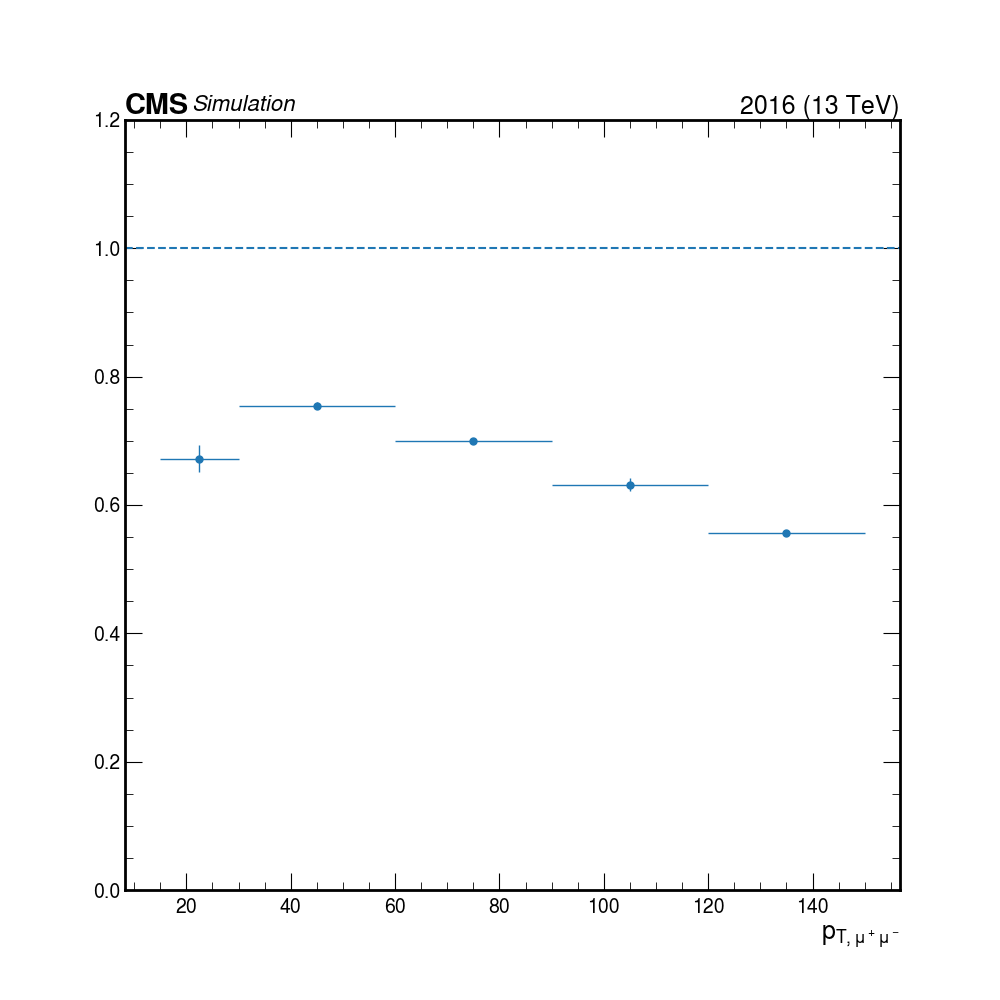
\includegraphics[width=0.44\textwidth]{figures/efficiency/eff_trigger_pt_2016.png}}}\hfill
  \subfloat[][]{\label{subfig:eff_trigger_rap_2016}%
    \fbox{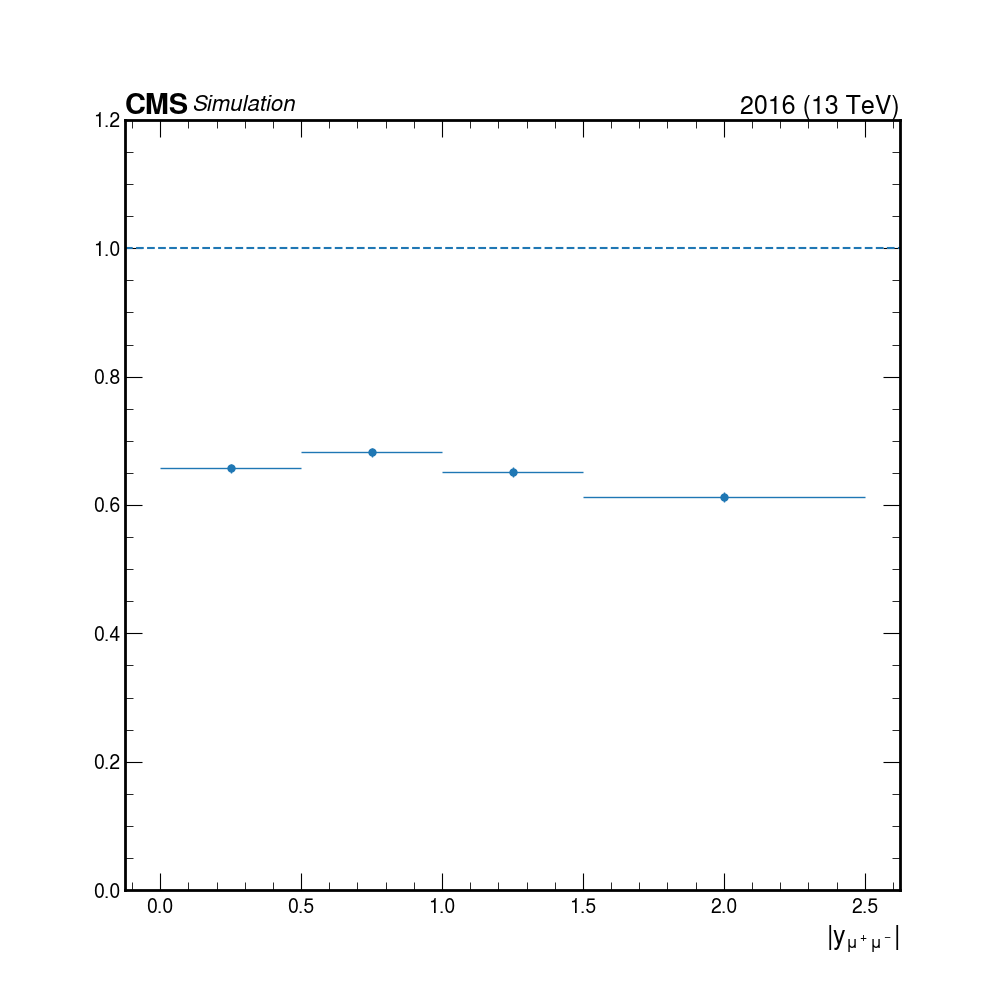
\includegraphics[width=0.44\textwidth]{figures/efficiency/eff_trigger_rap_2016.png}}}\hfill\\
  \subfloat[][]{\label{subfig:eff_trigger_2D_2016}%
    \fbox{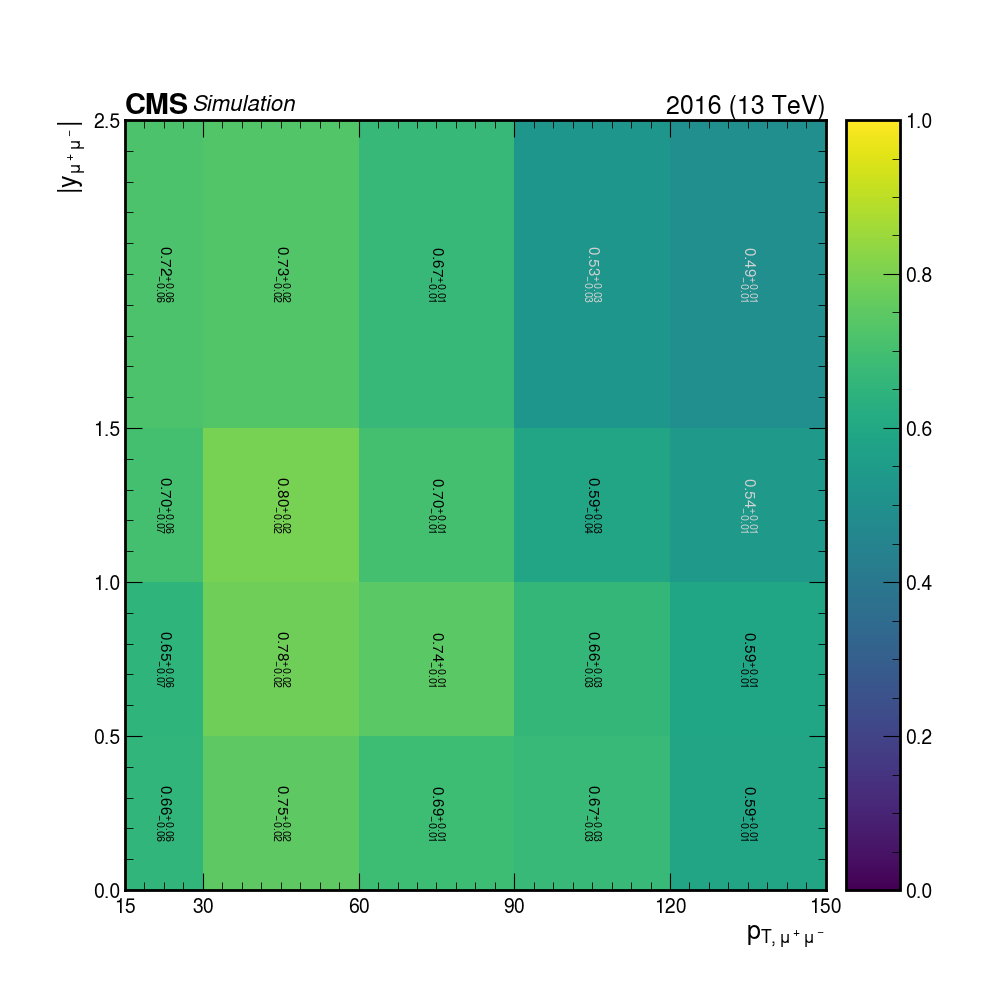
\includegraphics[width=0.44\textwidth]{figures/efficiency/eff_trigger_2016.png}}}\\
  \legend{Trigger efficiency extracted from the 2016 MC data sample. This efficiency is given with respect to the dimuon $p_T$ in (a), $y$ in (b), and in both $p_T$ and $y$ in (c). In (a) and (b). The horizontal dashed line is set to the upper limit of the efficiency.}
\end{figure}

\begin{figure}[H]{15cm}
  \caption{Trigger efficiency of the selected associated $\Upsilon +$ D$^*$ extracted from 2016 MC sample.}
  \label{fig:eff_asso_2016}
  \subfloat[][]{\label{subfig:eff_asso_pt_2016}%
    \fbox{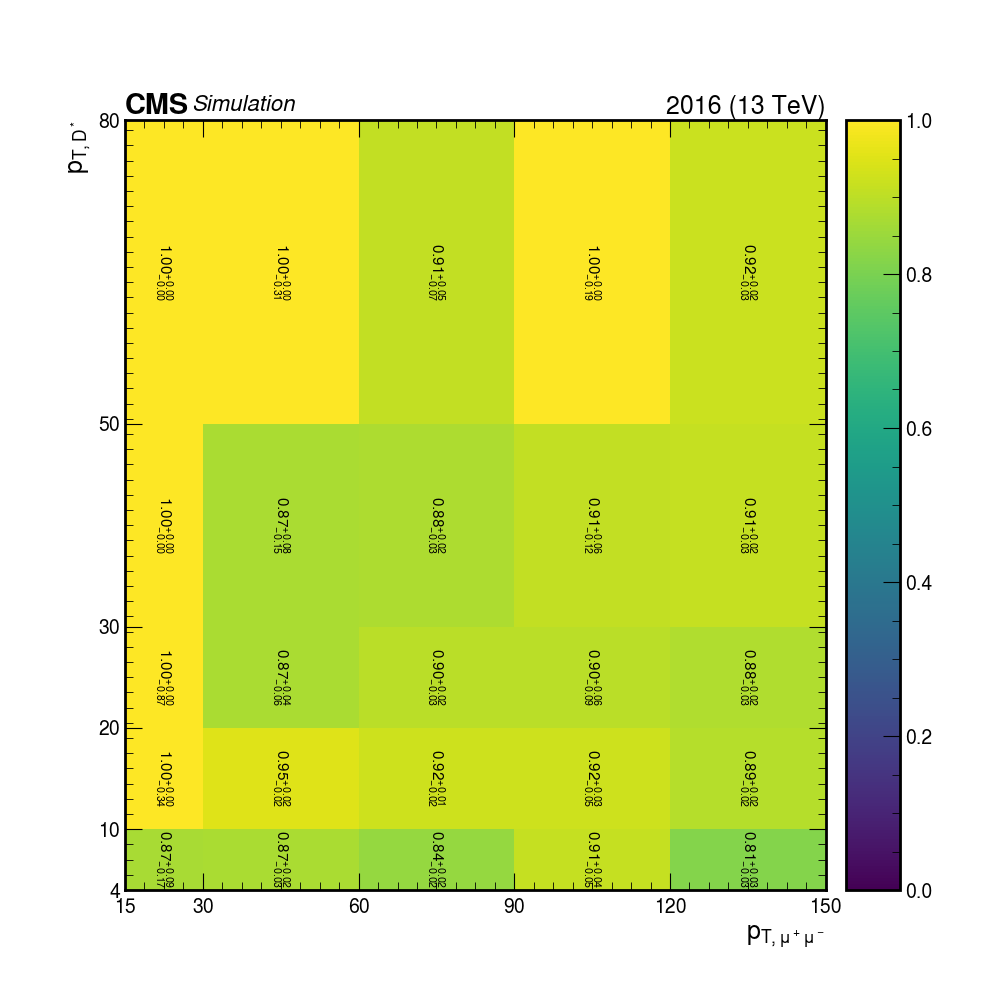
\includegraphics[width=0.44\textwidth]{figures/efficiency/eff_asso_pt_2016.png}}}\hfill
  \subfloat[][]{\label{subfig:eff_asso_rap_2016}%
    \fbox{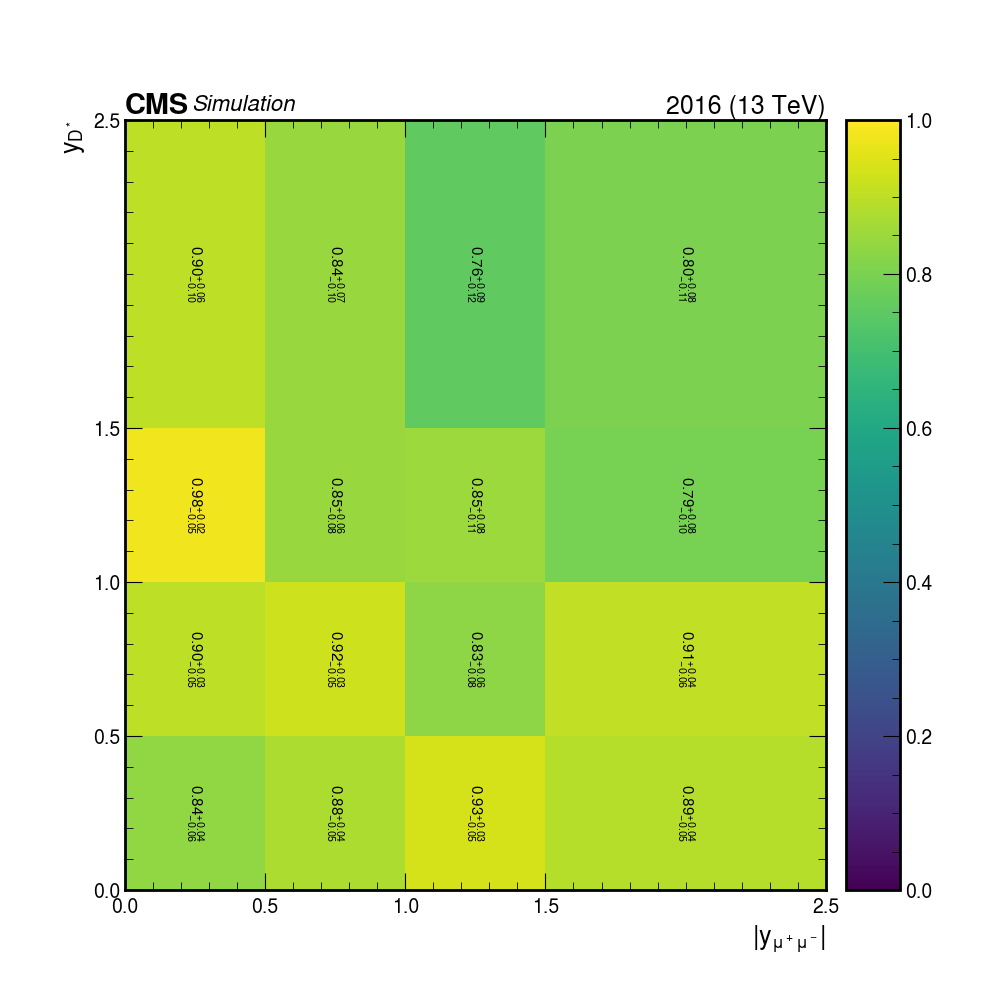
\includegraphics[width=0.44\textwidth]{figures/efficiency/eff_asso_rap_2016.png}}}\hfill\\
  \legend{Association efficiency extracted from the 2016 MC data sample. The efficiency maps are given with respect to the dimuon and D$^*$ $p_T$ in (a) and $y$ in (b).}
\end{figure}

\clearpage

\section{Efficiencies for sample 2017}

\begin{figure}[H]{15cm}
  \caption{$\Upsilon$ acceptance of the selected associated $\Upsilon +$ D$^*$ extracted from 2017 MC sample.}
  \label{fig:acc_dimu_2017}
  \subfloat[][]{\label{subfig:acc_dimu_pt_2017}%
    \fbox{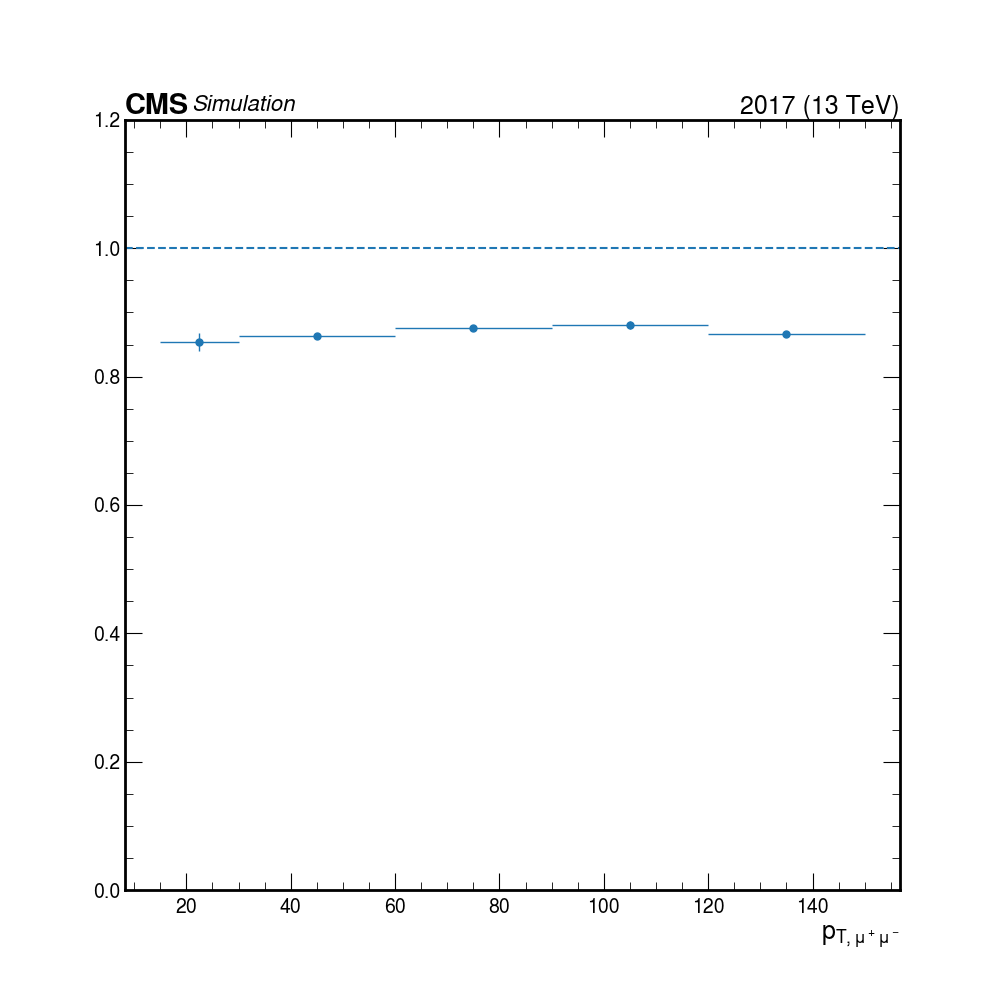
\includegraphics[width=0.44\textwidth]{figures/efficiency/acc_dimu_pt_2017.png}}}\hfill
  \subfloat[][]{\label{subfig:acc_dimu_rap_2017}%
    \fbox{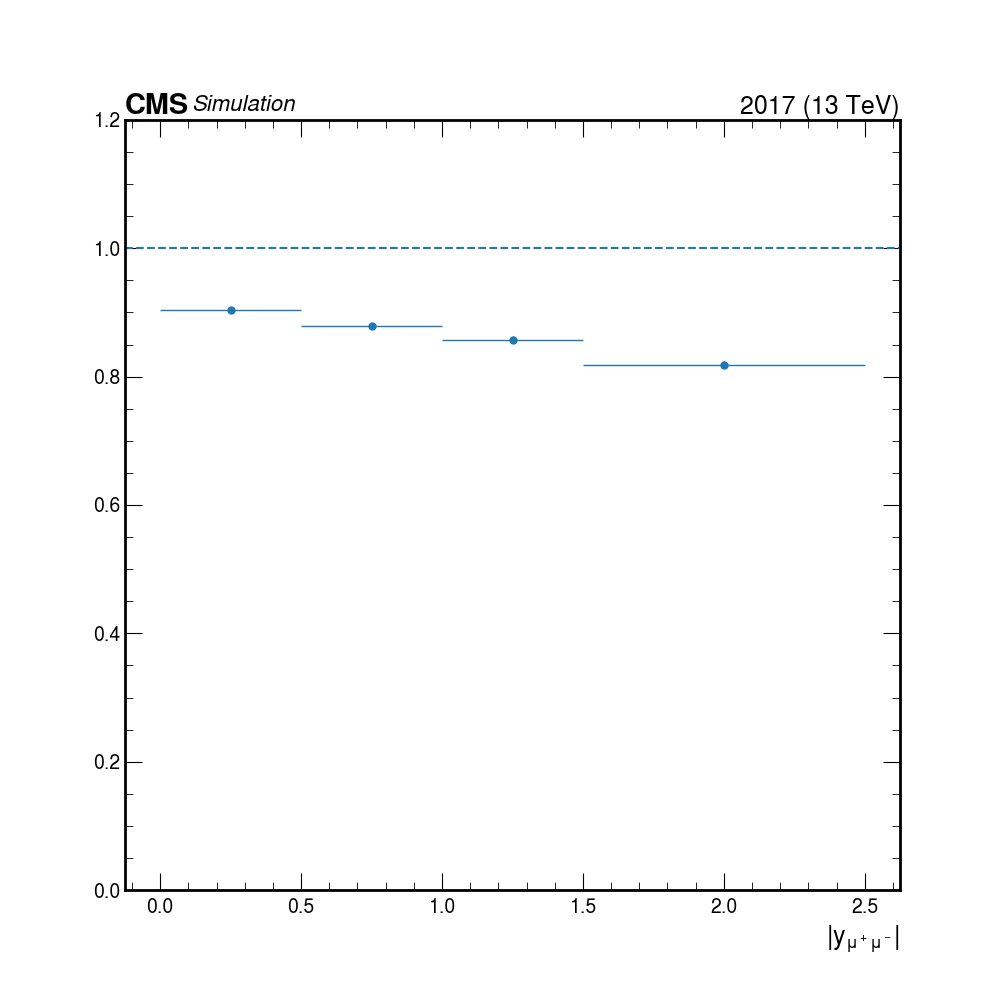
\includegraphics[width=0.44\textwidth]{figures/efficiency/acc_dimu_rap_2017.png}}}\hfill\\
  \subfloat[][]{\label{subfig:acc_dimu_2D_2017}%
    \fbox{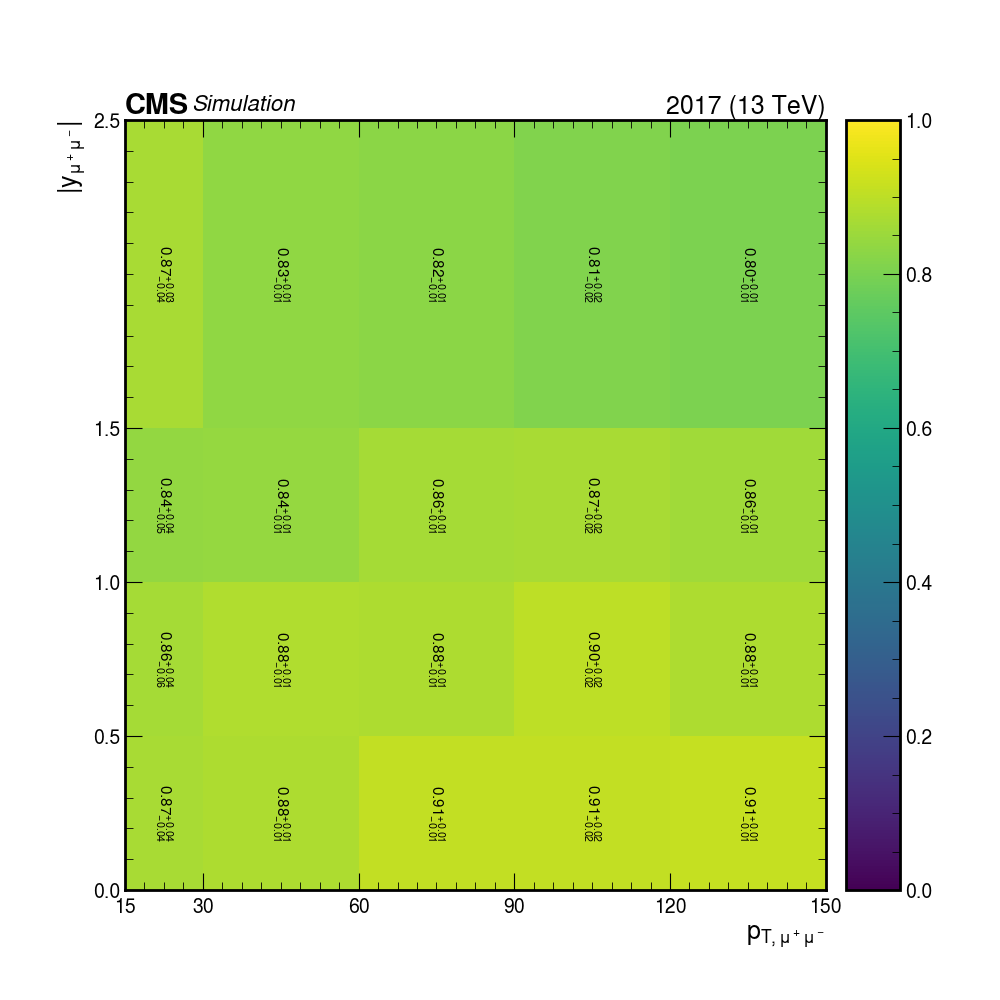
\includegraphics[width=0.44\textwidth]{figures/efficiency/acc_dimu_2017.png}}}\\
  \legend{$\Upsilon$ acceptance extracted from the 2017 MC data sample. The acceptance is given with respect to the dimuon $p_T$ in (a), $y$ in (b), and in both $p_T$ and $y$ in (c). In (a) and (b). The horizontal dashed line is set to the upper limit of the acceptance, one.}
\end{figure}

\begin{figure}[H]{15cm}
  \caption{D$^*$ acceptance of the selected associated $\Upsilon +$ D$^*$ extracted from 2017 MC sample.}
  \label{fig:acc_dstar_2017}
  \subfloat[][]{\label{subfig:acc_dstar_pt_2017}%
    \fbox{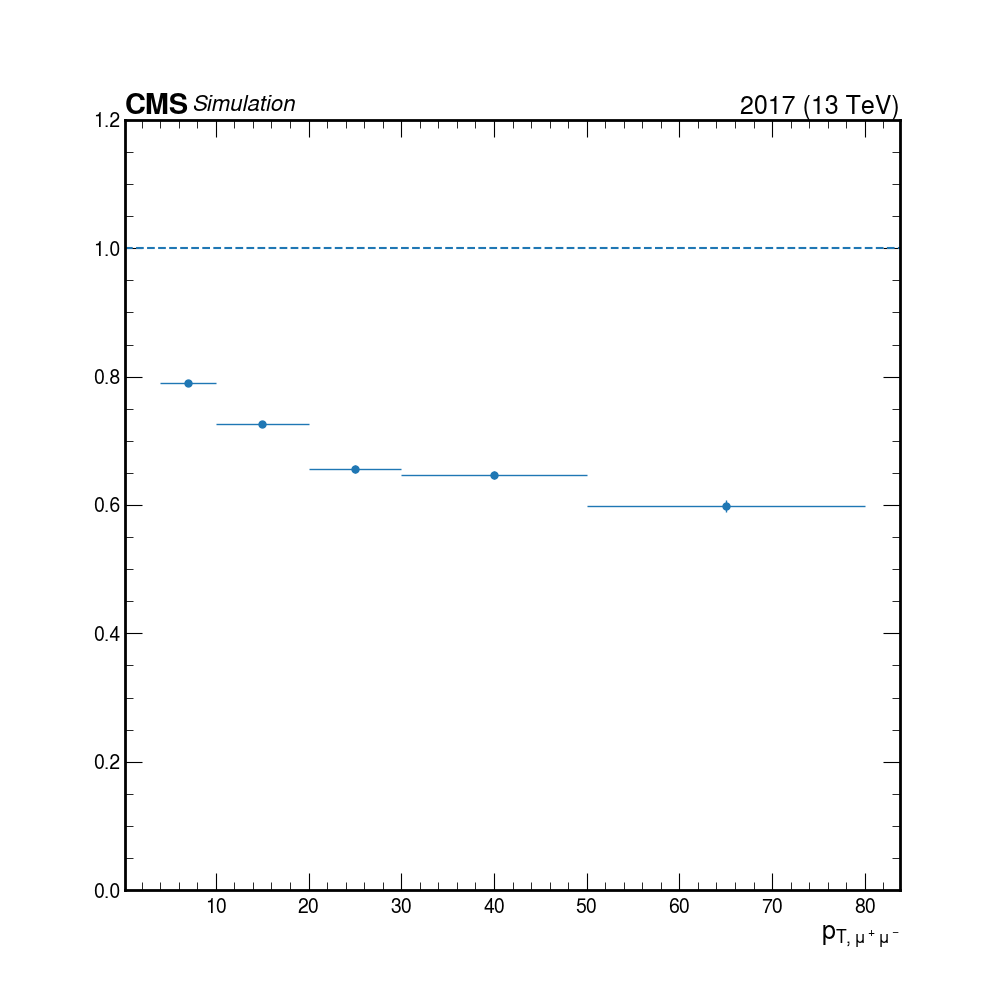
\includegraphics[width=0.44\textwidth]{figures/efficiency/acc_dstar_pt_2017.png}}}\hfill
  \subfloat[][]{\label{subfig:acc_dstar_rap_2017}%
    \fbox{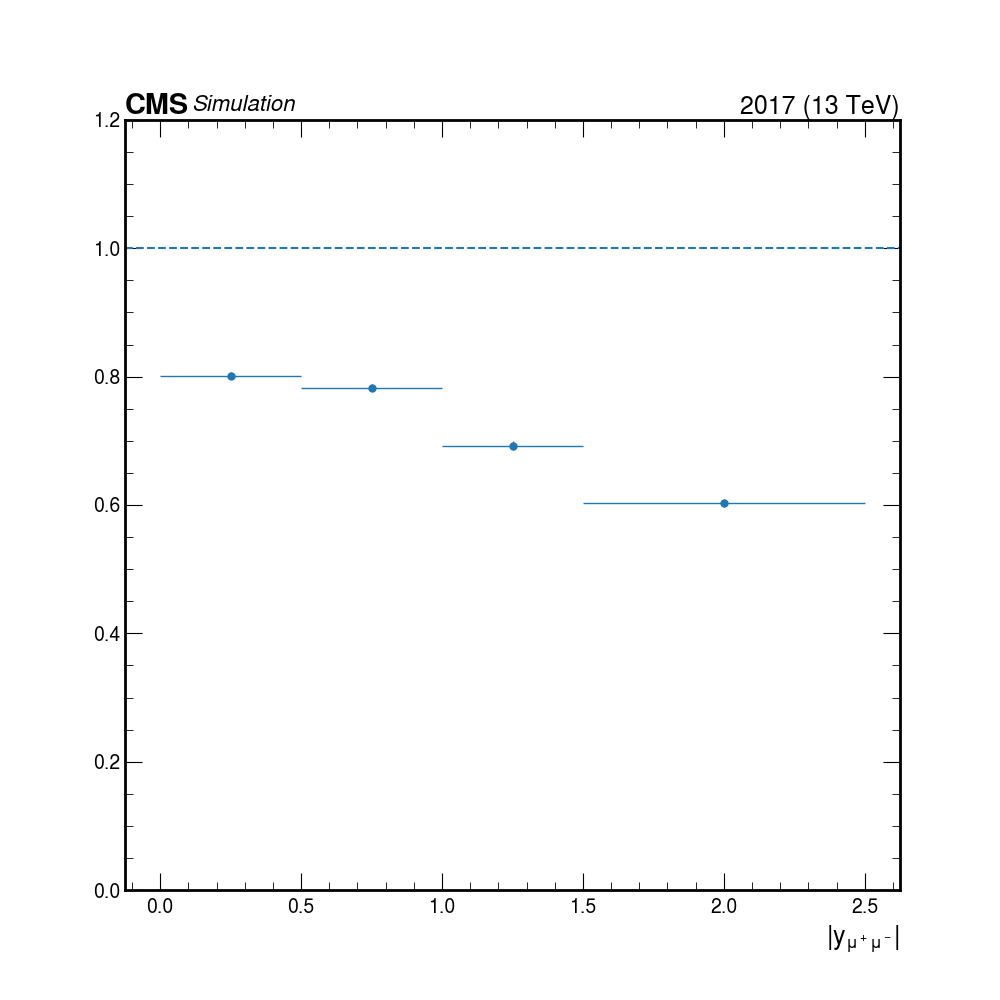
\includegraphics[width=0.44\textwidth]{figures/efficiency/acc_dstar_rap_2017.png}}}\hfill\\
  \subfloat[][]{\label{subfig:acc_dstar_2D_2017}%
    \fbox{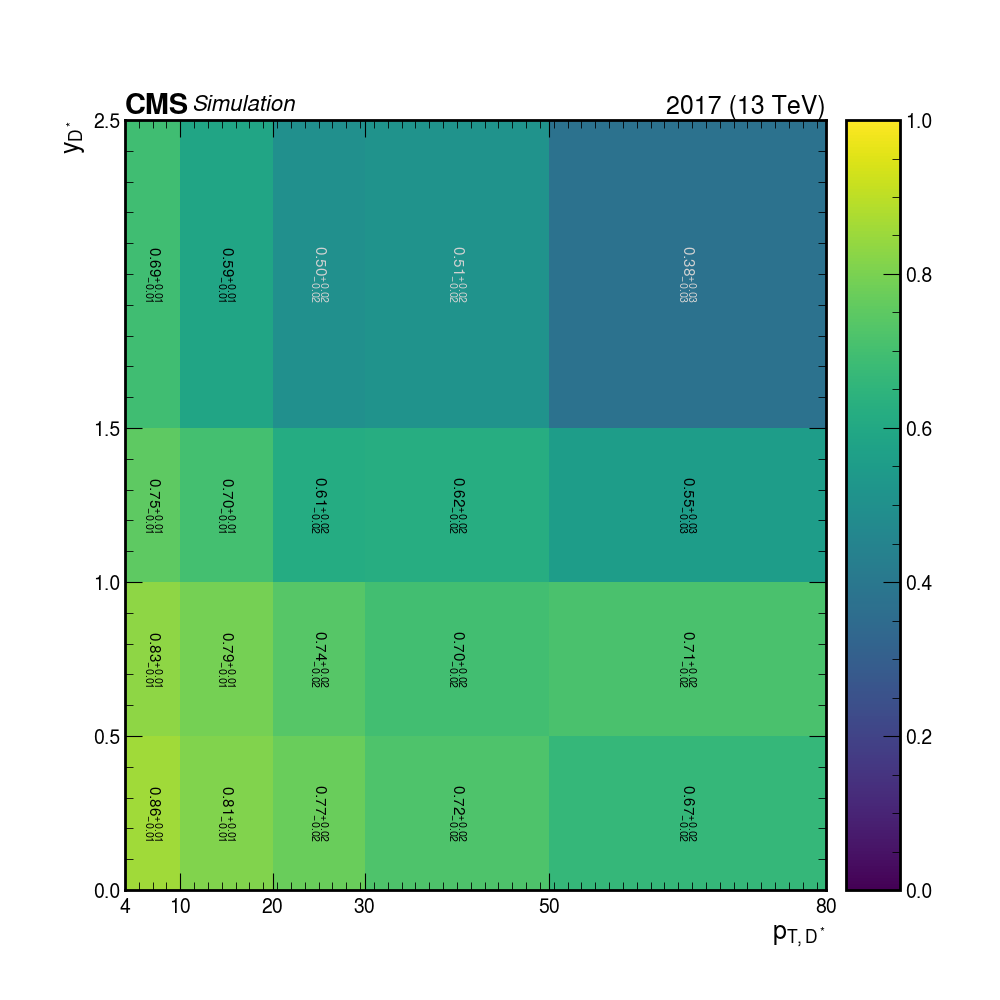
\includegraphics[width=0.44\textwidth]{figures/efficiency/acc_dstar_2017.png}}}\\
  \legend{D$^*$ acceptance extracted from the 2017 MC data sample. The acceptance is given with respect to the reconstructed D$^*$ $p_T$ in (a), $y$ in (b), and in both $p_T$ and $y$ in (c). In (a) and (b). The horizontal dashed line is set to the upper limit of the acceptance, one.}
\end{figure}

\begin{figure}[H]{15cm}
  \caption{$\Upsilon$ selection cuts efficiency of the selected associated $\Upsilon +$ D$^*$ extracted from 2017 MC sample.}
  \label{fig:eff_cuts_dimu_2017}
  \subfloat[][]{\label{subfig:eff_cuts_dimu_pt_2017}%
  \fbox{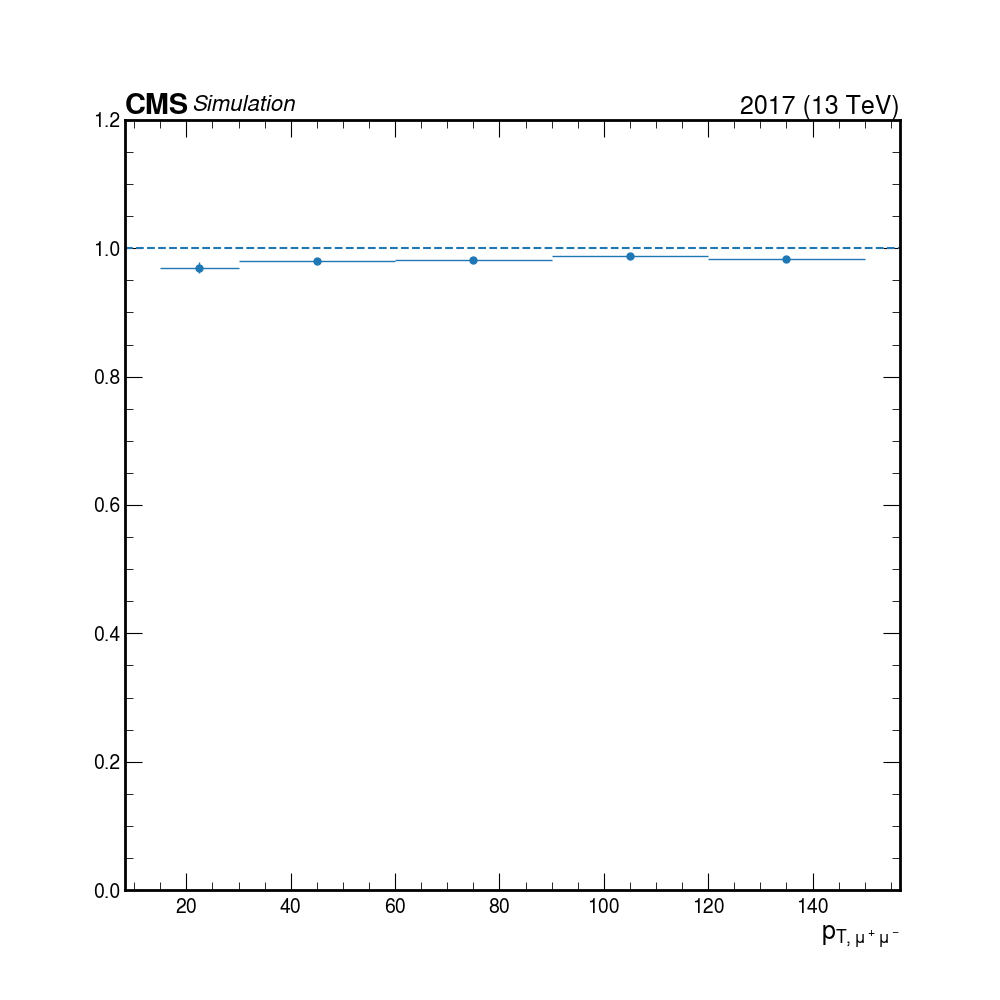
\includegraphics[width=0.44\textwidth]{figures/efficiency/eff_cuts_dimu_pt_2017.png}}}\hfill
  \subfloat[][]{\label{subfig:eff_cuts_dimu_rap_2017}%
  \fbox{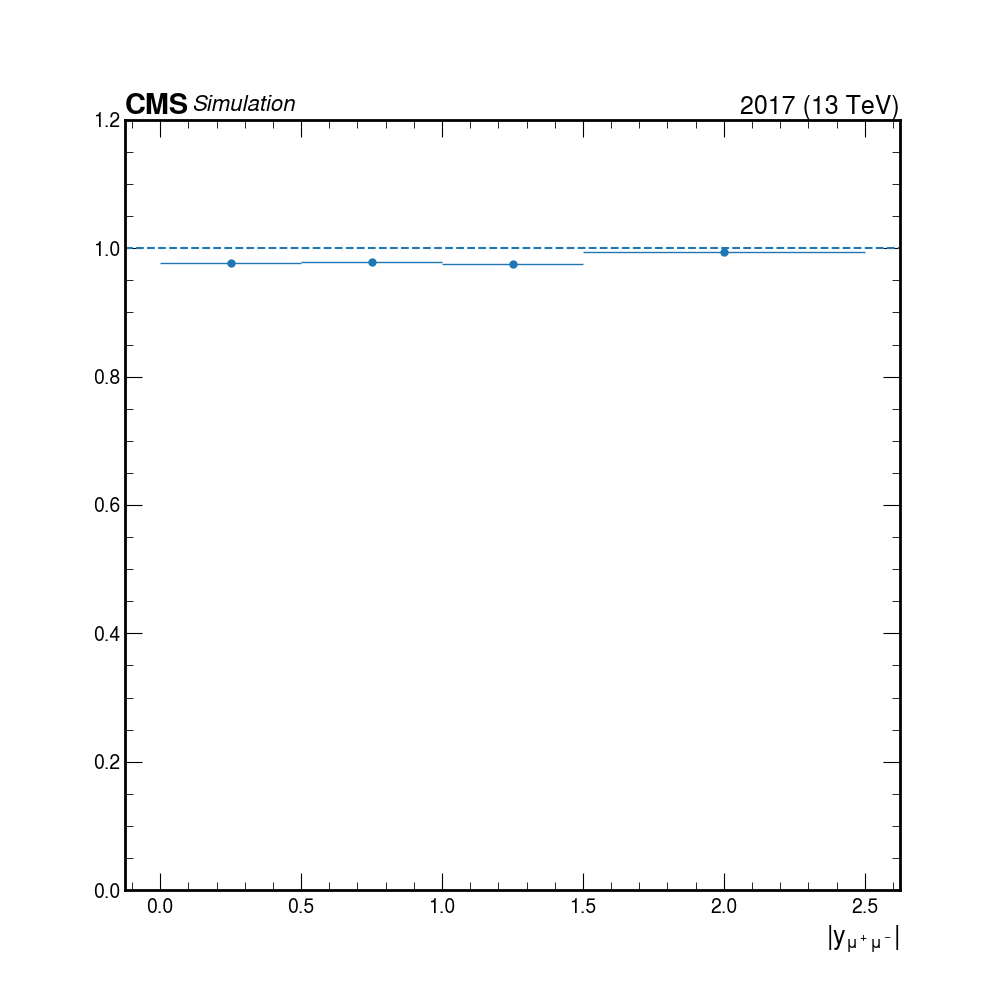
\includegraphics[width=0.44\textwidth]{figures/efficiency/eff_cuts_dimu_rap_2017.png}}}\hfill\\
  \subfloat[][]{\label{subfig:eff_cuts_dimu_2D_2017}%
  \fbox{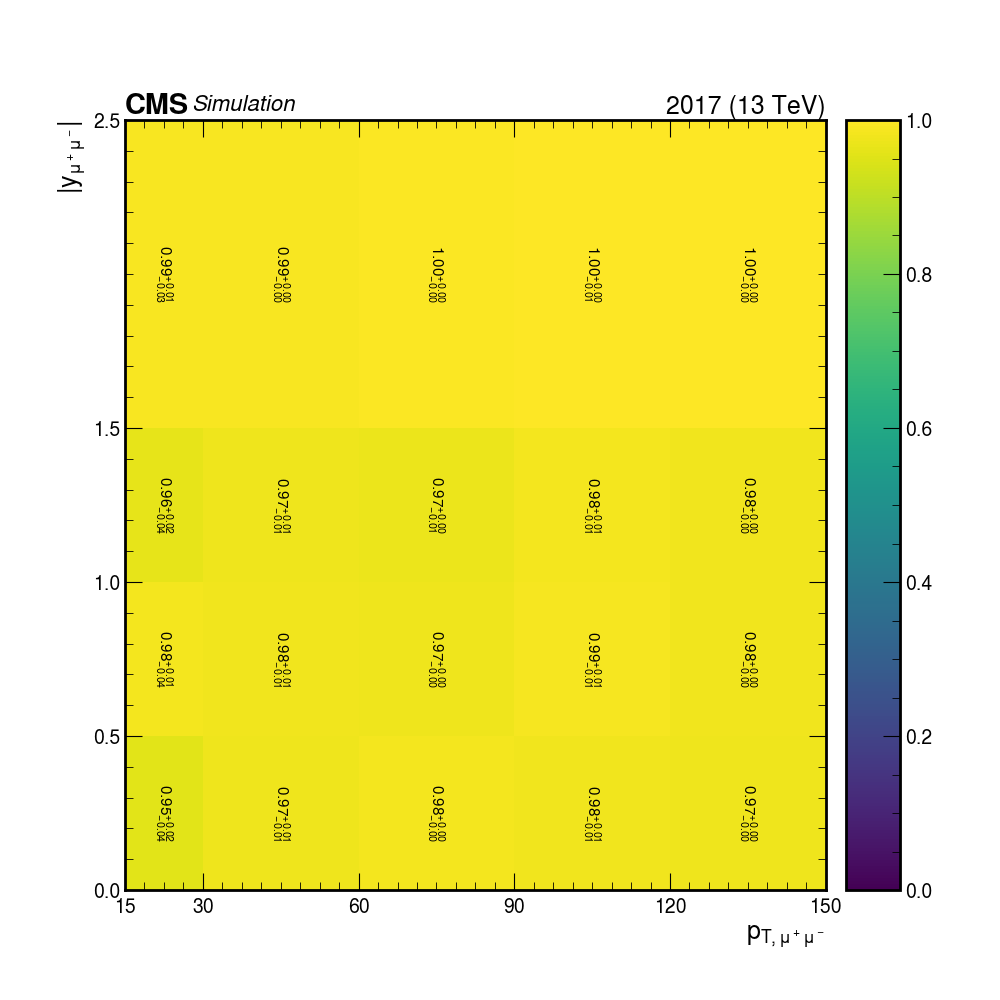
\includegraphics[width=0.44\textwidth]{figures/efficiency/eff_cuts_dimu_2017.png}}}\\
  \legend{$\Upsilon$ selection cuts efficiency extracted from the 2017 MC data sample. This efficiency is given with respect to the dimuon $p_T$ in (a), $y$ in (b), and in both $p_T$ and $y$ in (c). In (a) and (b). The horizontal dashed line is set to the upper limit of the efficiency.}
\end{figure}

\begin{figure}[H]{15cm}
  \caption{D$^*$ selection cuts efficiency of the selected associated $\Upsilon +$ D$^*$ extracted from 2017 MC sample.}
  \label{fig:eff_cuts_dstar_2017}
  \subfloat[][]{\label{subfig:eff_cuts_dstar_pt_2017}%
    \fbox{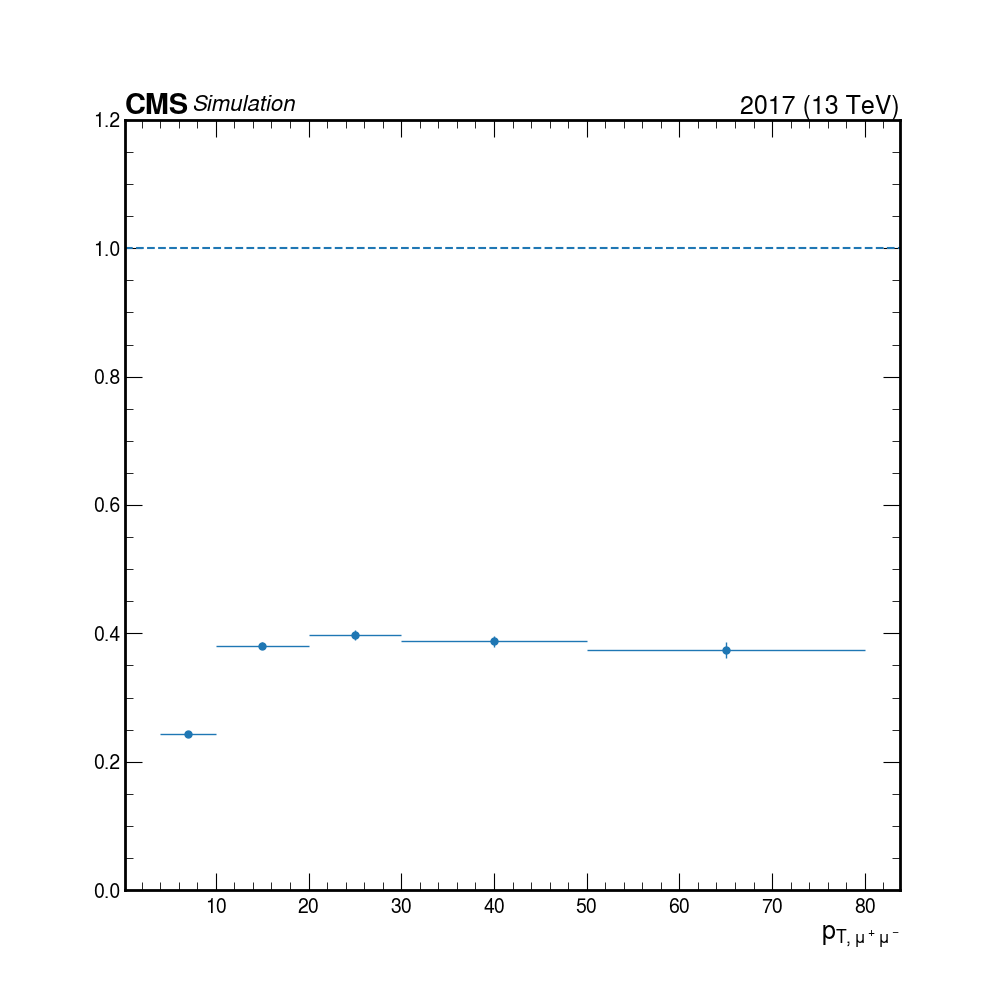
\includegraphics[width=0.44\textwidth]{figures/efficiency/eff_cuts_dstar_pt_2017.png}}}\hfill
  \subfloat[][]{\label{subfig:eff_cuts_dstar_rap_2017}%
    \fbox{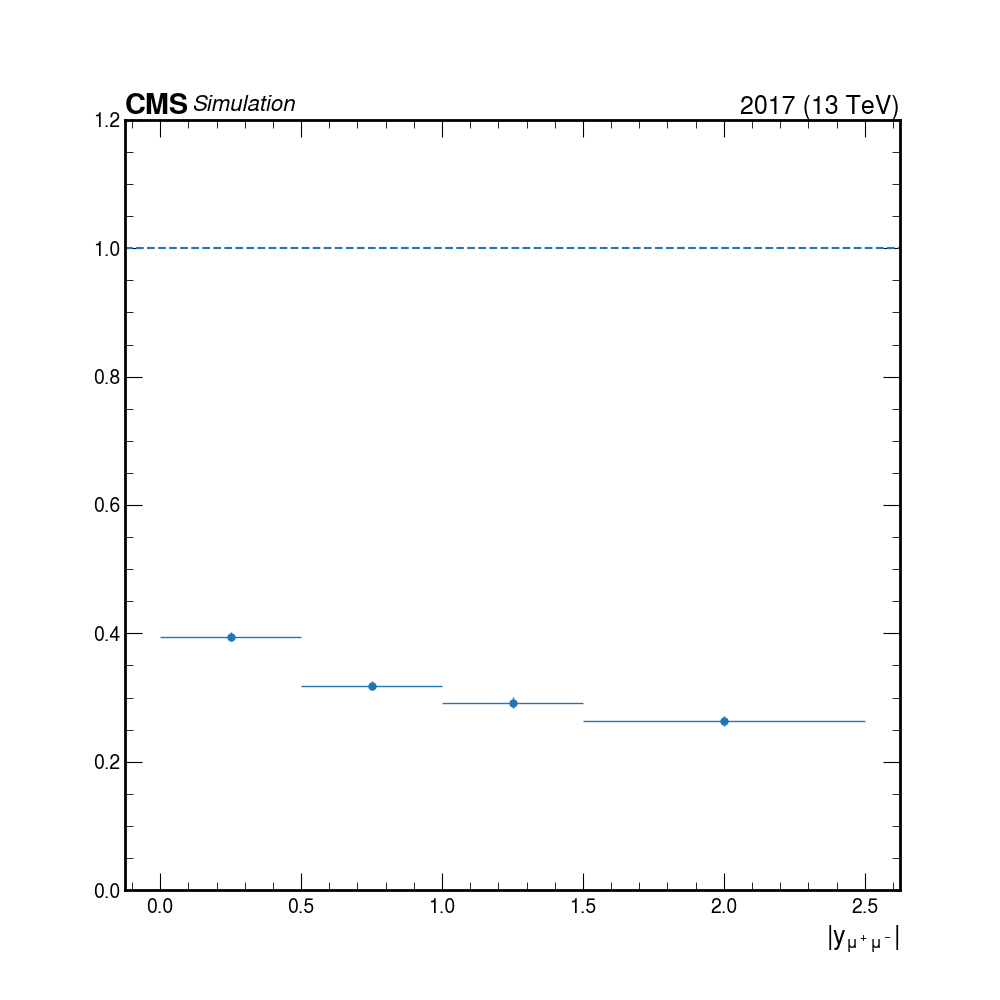
\includegraphics[width=0.44\textwidth]{figures/efficiency/eff_cuts_dstar_rap_2017.png}}}\hfill\\
  \subfloat[][]{\label{subfig:eff_cuts_dstar_2D_2017}%
    \fbox{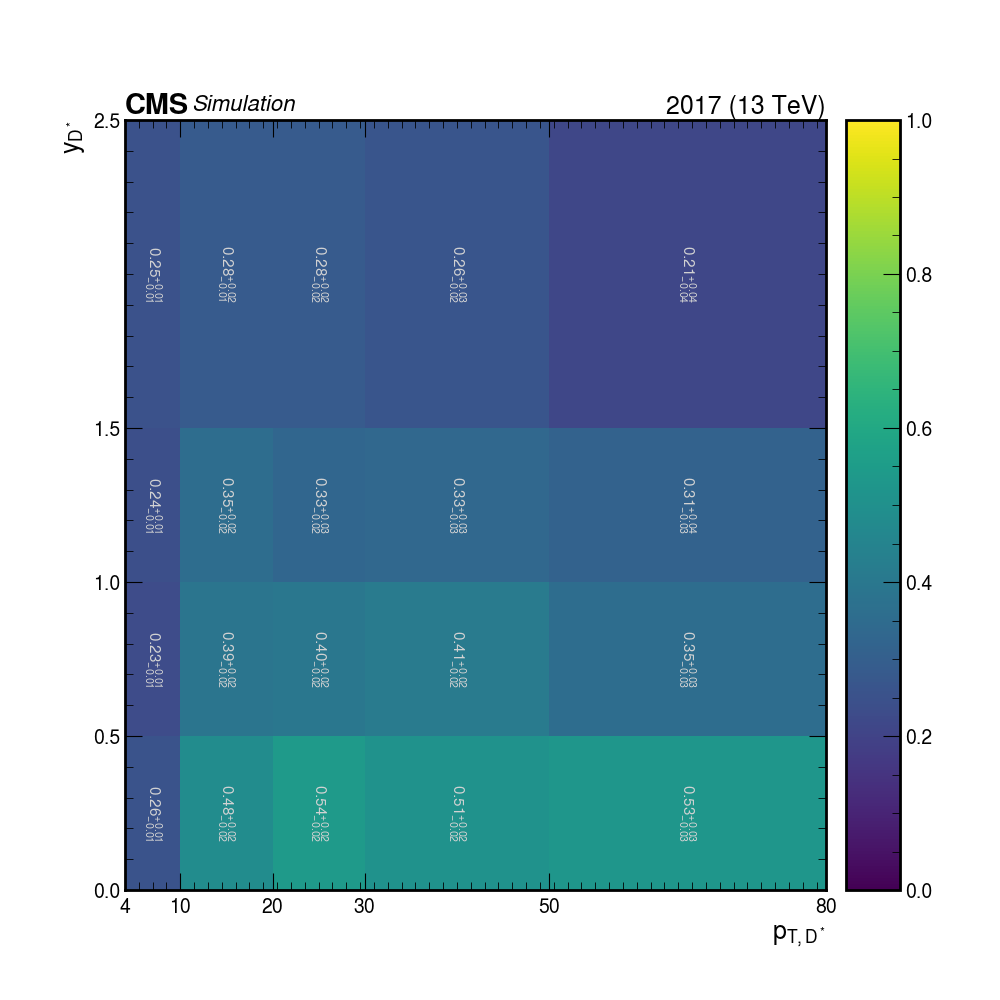
\includegraphics[width=0.44\textwidth]{figures/efficiency/eff_cuts_dstar_2017.png}}}\\
  \legend{D$^*$ selection cuts efficiency extracted from the 2017 MC data sample. This efficiency is given with respect to the D$^*$ $p_T$ in (a), $y$ in (b), and in both $p_T$ and $y$ in (c). In (a) and (b). The horizontal dashed line is set to the upper limit of the efficiency.}
\end{figure}

\begin{figure}[H]{15cm}
  \caption{Trigger efficiency of the selected associated $\Upsilon +$ D$^*$ extracted from 2017 MC sample.}
  \label{fig:eff_trigger_2017}
  \subfloat[][]{\label{subfig:eff_trigger_pt_2017}%
    \fbox{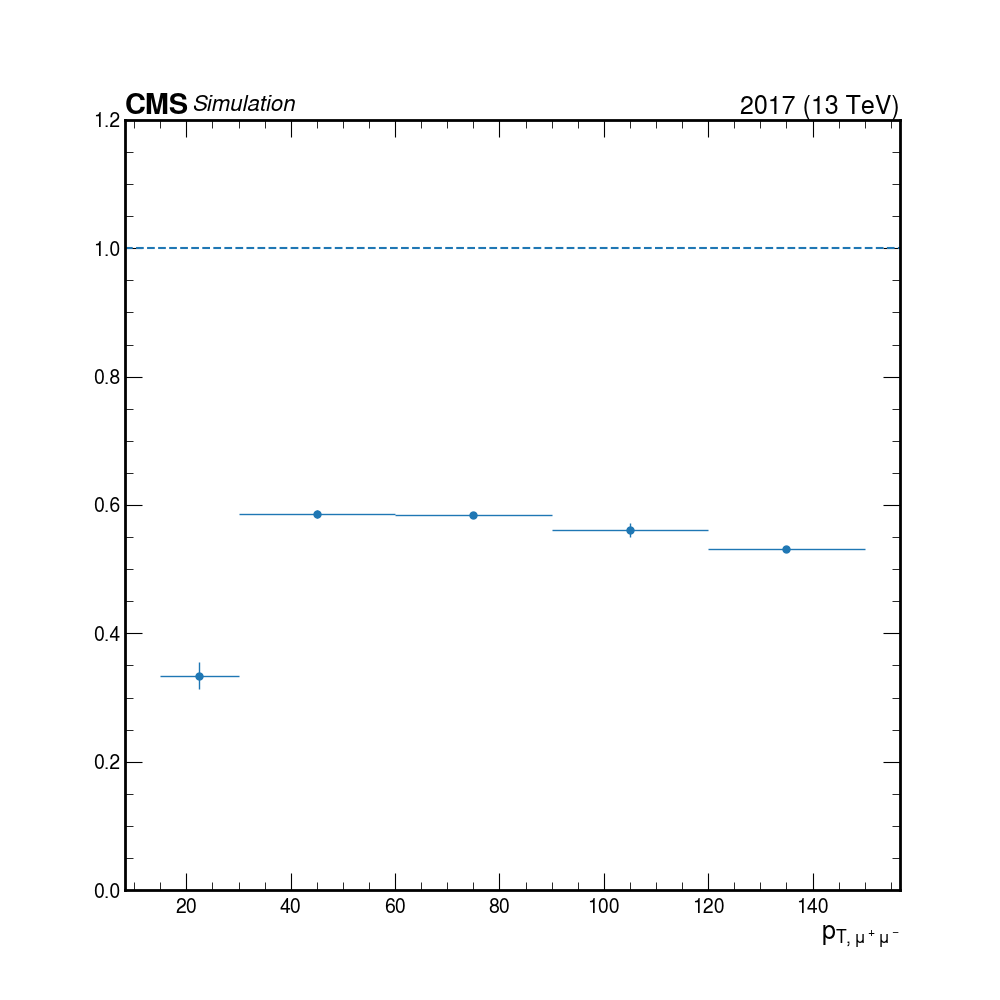
\includegraphics[width=0.44\textwidth]{figures/efficiency/eff_trigger_pt_2017.png}}}\hfill
  \subfloat[][]{\label{subfig:eff_trigger_rap_2017}%
    \fbox{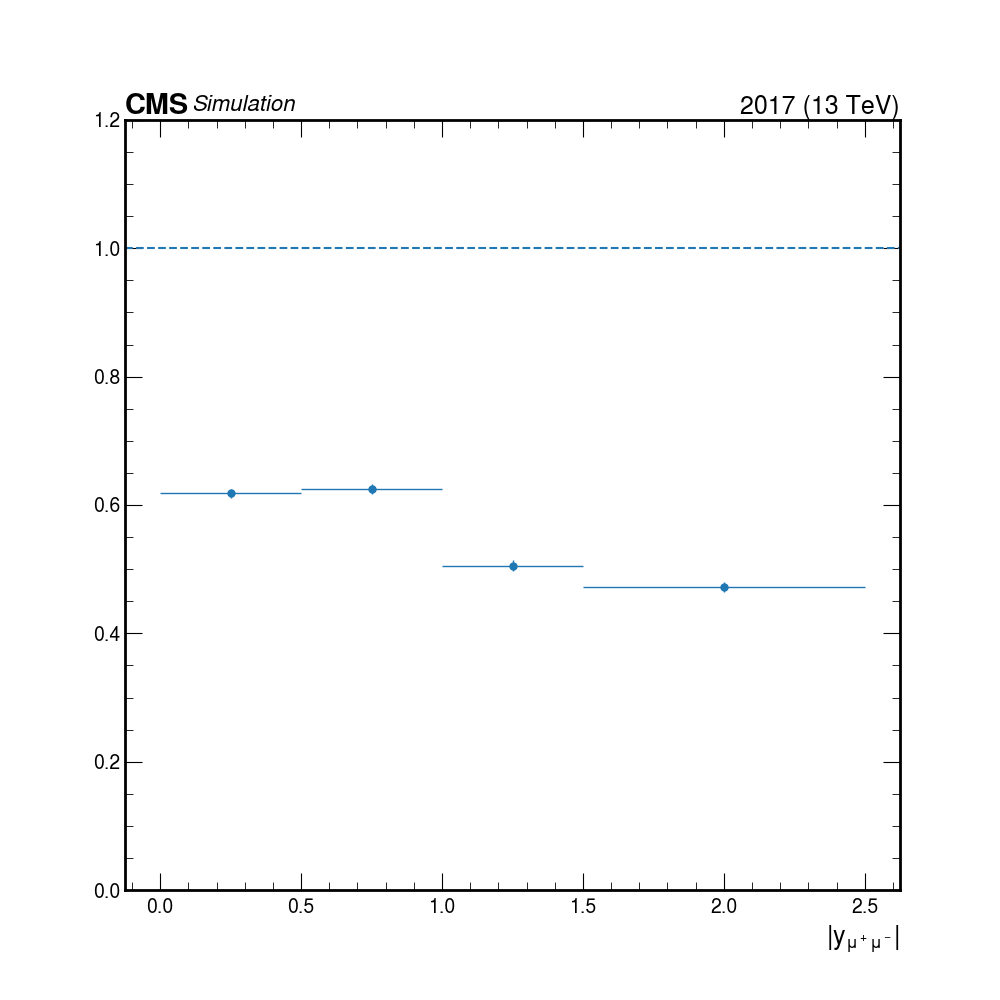
\includegraphics[width=0.44\textwidth]{figures/efficiency/eff_trigger_rap_2017.png}}}\hfill\\
  \subfloat[][]{\label{subfig:eff_trigger_2D_2017}%
    \fbox{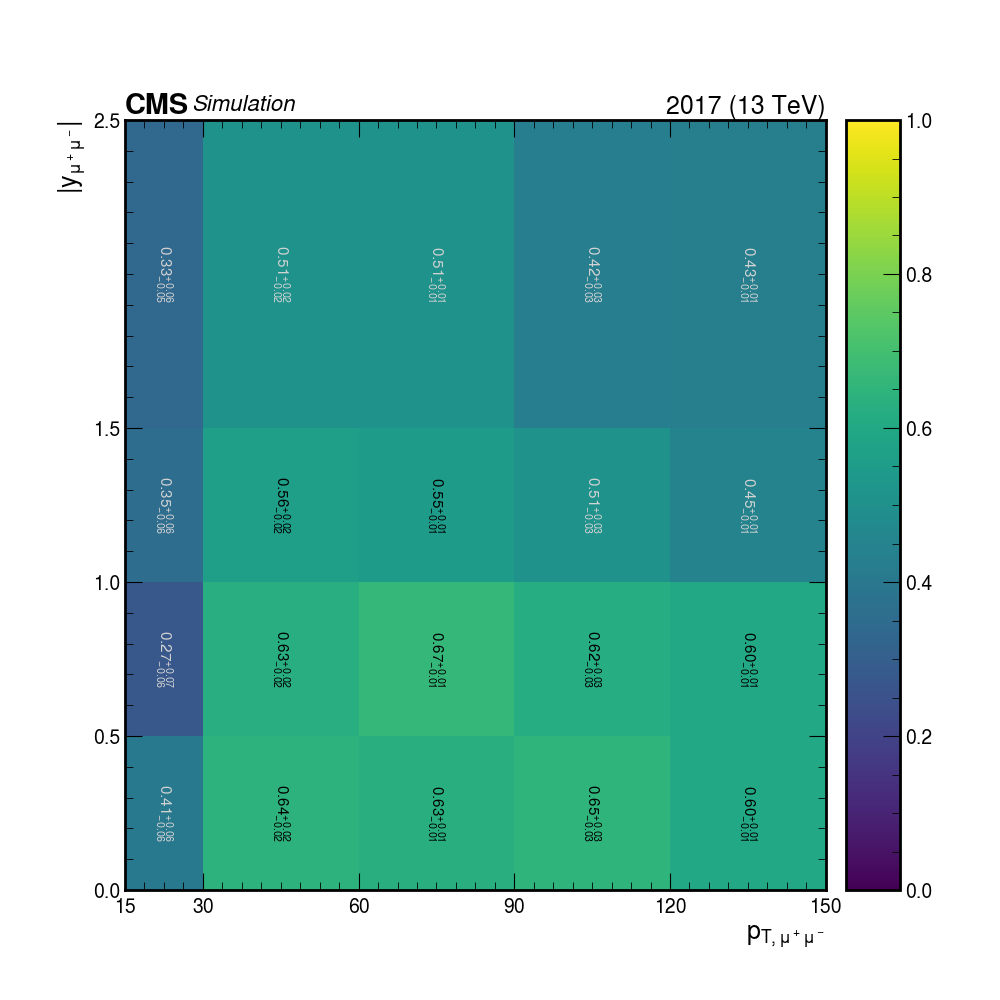
\includegraphics[width=0.44\textwidth]{figures/efficiency/eff_trigger_2017.png}}}\\
  \legend{Trigger efficiency extracted from the 2017 MC data sample. This efficiency is given with respect to the dimuon $p_T$ in (a), $y$ in (b), and in both $p_T$ and $y$ in (c). In (a) and (b). The horizontal dashed line is set to the upper limit of the efficiency.}
\end{figure}

\begin{figure}[H]{15cm}
  \caption{Trigger efficiency of the selected associated $\Upsilon +$ D$^*$ extracted from 2017 MC sample.}
  \label{fig:eff_asso_2017}
  \subfloat[][]{\label{subfig:eff_asso_pt_2017}%
    \fbox{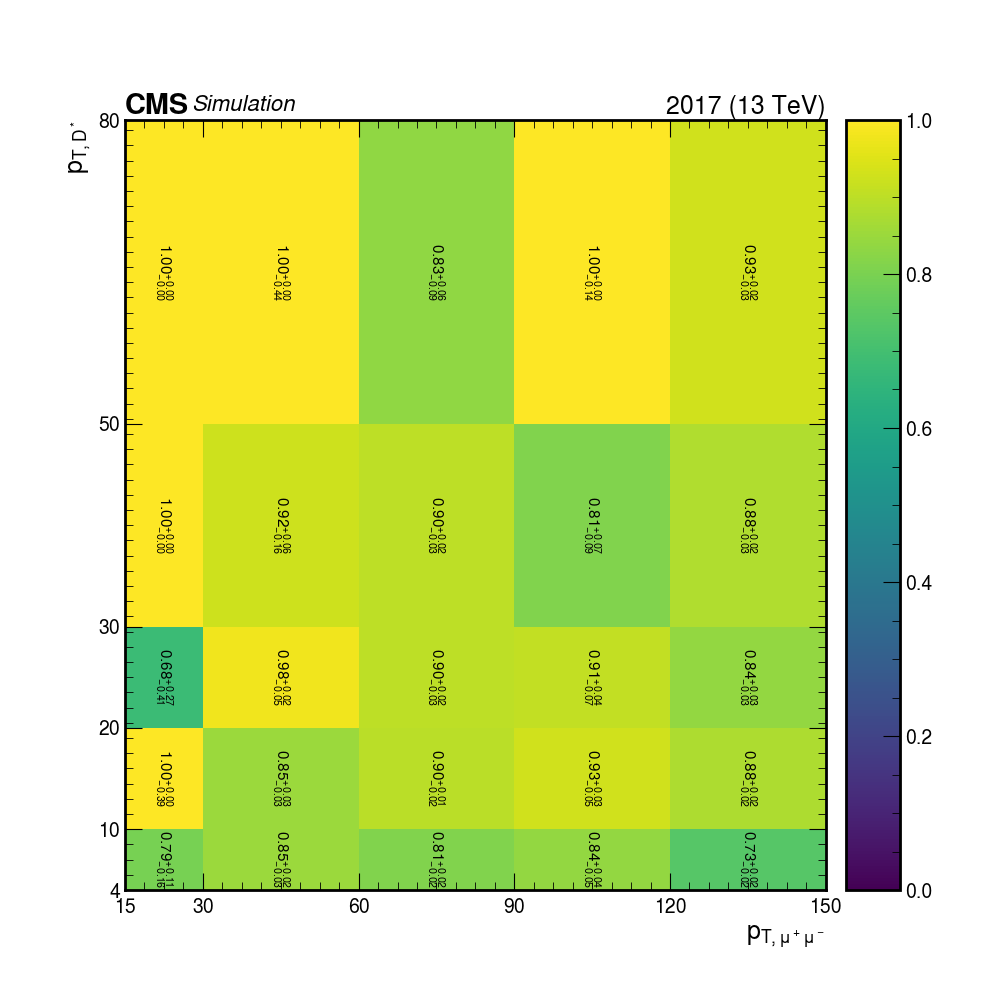
\includegraphics[width=0.44\textwidth]{figures/efficiency/eff_asso_pt_2017.png}}}\hfill
  \subfloat[][]{\label{subfig:eff_asso_rap_2017}%
    \fbox{\includegraphics[width=0.44\textwidth]{figures/efficiency/eff_asso_rap_2017.png}}}\hfill\\
  \legend{Association efficiency extracted from the 2017 MC data sample. The efficiency maps are given with respect to the dimuon and D$^*$ $p_T$ in (a) and $y$ in (b).}
\end{figure}

\clearpage

\section{Efficiencies for sample 2018}

\begin{figure}[H]{15cm}
  \caption{$\Upsilon$ acceptance of the selected associated $\Upsilon +$ D$^*$ extracted from 2018 MC sample.}
  \label{fig:acc_dimu_2018}
  \subfloat[][]{\label{subfig:acc_dimu_pt_2018}%
    \fbox{\includegraphics[width=0.44\textwidth]{figures/efficiency/acc_dimu_pt_2018.png}}}\hfill
  \subfloat[][]{\label{subfig:acc_dimu_rap_2018}%
    \fbox{\includegraphics[width=0.44\textwidth]{figures/efficiency/acc_dimu_rap_2018.png}}}\hfill\\
  \subfloat[][]{\label{subfig:acc_dimu_2D_2018}%
    \fbox{\includegraphics[width=0.44\textwidth]{figures/efficiency/acc_dimu_2018.png}}}\\
  \legend{$\Upsilon$ acceptance extracted from the 2018 MC data sample. The acceptance is given with respect to the dimuon $p_T$ in (a), $y$ in (b), and in both $p_T$ and $y$ in (c). In (a) and (b). The horizontal dashed line is set to the upper limit of the acceptance, one.}
\end{figure}

\begin{figure}[H]{15cm}
  \caption{D$^*$ acceptance of the selected associated $\Upsilon +$ D$^*$ extracted from 2018 MC sample.}
  \label{fig:acc_dstar_2018}
  \subfloat[][]{\label{subfig:acc_dstar_pt_2018}%
    \fbox{\includegraphics[width=0.44\textwidth]{figures/efficiency/acc_dstar_pt_2018.png}}}\hfill
  \subfloat[][]{\label{subfig:acc_dstar_rap_2018}%
    \fbox{\includegraphics[width=0.44\textwidth]{figures/efficiency/acc_dstar_rap_2018.png}}}\hfill\\
  \subfloat[][]{\label{subfig:acc_dstar_2D_2018}%
    \fbox{\includegraphics[width=0.44\textwidth]{figures/efficiency/acc_dstar_2018.png}}}\\
  \legend{D$^*$ acceptance extracted from the 2018 MC data sample. The acceptance is given with respect to the reconstructed D$^*$ $p_T$ in (a), $y$ in (b), and in both $p_T$ and $y$ in (c). In (a) and (b). The horizontal dashed line is set to the upper limit of the acceptance, one.}
\end{figure}

\begin{figure}[H]{15cm}
  \caption{$\Upsilon$ selection cuts efficiency of the selected associated $\Upsilon +$ D$^*$ extracted from 2018 MC sample.}
  \label{fig:eff_cuts_dimu_2018}
  \subfloat[][]{\label{subfig:eff_cuts_dimu_pt_2018}%
  \fbox{\includegraphics[width=0.44\textwidth]{figures/efficiency/eff_cuts_dimu_pt_2018.png}}}\hfill
  \subfloat[][]{\label{subfig:eff_cuts_dimu_rap_2018}%
  \fbox{\includegraphics[width=0.44\textwidth]{figures/efficiency/eff_cuts_dimu_rap_2018.png}}}\hfill\\
  \subfloat[][]{\label{subfig:eff_cuts_dimu_2D_2018}%
  \fbox{\includegraphics[width=0.44\textwidth]{figures/efficiency/eff_cuts_dimu_2018.png}}}\\
  \legend{$\Upsilon$ selection cuts efficiency extracted from the 2018 MC data sample. This efficiency is given with respect to the dimuon $p_T$ in (a), $y$ in (b), and in both $p_T$ and $y$ in (c). In (a) and (b). The horizontal dashed line is set to the upper limit of the efficiency.}
\end{figure}

\begin{figure}[H]{15cm}
  \caption{D$^*$ selection cuts efficiency of the selected associated $\Upsilon +$ D$^*$ extracted from 2018 MC sample.}
  \label{fig:eff_cuts_dstar_2018}
  \subfloat[][]{\label{subfig:eff_cuts_dstar_pt_2018}%
    \fbox{\includegraphics[width=0.44\textwidth]{figures/efficiency/eff_cuts_dstar_pt_2018.png}}}\hfill
  \subfloat[][]{\label{subfig:eff_cuts_dstar_rap_2018}%
    \fbox{\includegraphics[width=0.44\textwidth]{figures/efficiency/eff_cuts_dstar_rap_2018.png}}}\hfill\\
  \subfloat[][]{\label{subfig:eff_cuts_dstar_2D_2018}%
    \fbox{\includegraphics[width=0.44\textwidth]{figures/efficiency/eff_cuts_dstar_2018.png}}}\\
  \legend{D$^*$ selection cuts efficiency extracted from the 2018 MC data sample. This efficiency is given with respect to the D$^*$ $p_T$ in (a), $y$ in (b), and in both $p_T$ and $y$ in (c). In (a) and (b). The horizontal dashed line is set to the upper limit of the efficiency.}
\end{figure}

\begin{figure}[H]{15cm}
  \caption{Trigger efficiency of the selected associated $\Upsilon +$ D$^*$ extracted from 2018 MC sample.}
  \label{fig:eff_trigger_2018}
  \subfloat[][]{\label{subfig:eff_trigger_pt_2018}%
    \fbox{\includegraphics[width=0.44\textwidth]{figures/efficiency/eff_trigger_pt_2018.png}}}\hfill
  \subfloat[][]{\label{subfig:eff_trigger_rap_2018}%
    \fbox{\includegraphics[width=0.44\textwidth]{figures/efficiency/eff_trigger_rap_2018.png}}}\hfill\\
  \subfloat[][]{\label{subfig:eff_trigger_2D_2018}%
    \fbox{\includegraphics[width=0.44\textwidth]{figures/efficiency/eff_trigger_2018.png}}}\\
  \legend{Trigger efficiency extracted from the 2018 MC data sample. This efficiency is given with respect to the dimuon $p_T$ in (a), $y$ in (b), and in both $p_T$ and $y$ in (c). In (a) and (b). The horizontal dashed line is set to the upper limit of the efficiency.}
\end{figure}

\begin{figure}[H]{15cm}
  \caption{Trigger efficiency of the selected associated $\Upsilon +$ D$^*$ extracted from 2018 MC sample.}
  \label{fig:eff_asso_2018}
  \subfloat[][]{\label{subfig:eff_asso_pt_2018}%
    \fbox{\includegraphics[width=0.44\textwidth]{figures/efficiency/eff_asso_pt_2018.png}}}\hfill
  \subfloat[][]{\label{subfig:eff_asso_rap_2018}%
    \fbox{\includegraphics[width=0.44\textwidth]{figures/efficiency/eff_asso_rap_2018.png}}}\hfill\\
  \legend{Association efficiency extracted from the 2018 MC data sample. The efficiency maps are given with respect to the dimuon and D$^*$ $p_T$ in (a) and $y$ in (b).}
\end{figure}